\input{"header.tex"}



%Here is some text, where we use APC.\nomenclature{APC}{antigeen-presenterende cel}

%\printnomenclature

% -----------------------------------------------------------------------------
% Introduction and research problem

\chapter{Introduction to Neutrino Physics}
\label{c:theoryIntro}

This chapter is aimed at giving an introduction to the physics used in the thesis.

\section{Research Goals}
This research aims to construct a prototype Magnetized Iron Neutrino Detector (MIND) at the European Organization for Nuclear Research (CERN) and understand the performance of the detector to reconstruct charged particle tracks at a test beam at CERN and neutrino interactions at a neutrino beam at the JPARC facility in Japan.

\section{Theory}\label{section:Theory}
While measuring radioactive beta decay in the first two decades of the 20th century, physicists discovered what was then an anomaly. At the time it was thought that beta decay occurred as a two body process in which a neutron ($n$) decays to a proton ($p$) and electron ($e^-$). If this were the case, the energy of the proton and electron should be discrete and add up to the energy of neutron. However experiments showed that the electron could have a continuous spectrum of energy values, violating the energy conservation law, as seen in \FigRef{fig:betaeng}. In order to solve this anomaly, a third particle, the neutrino ($\nu$), was postulated by Wolfgang Pauli \cite{4Pauli:Online} and then incorporated into the beta decay by Enrico Fermi \cite{5Wilson}. The neutrino was postulated as a neutral particle with mass of less than 1\% of the proton mass and a spin of 1/2. For consistency, the particle used in the beta decay was changed to be noted as the antineutrino with the electron flavour, or just electron antineutrino $\bar{\nu_e}$. The addition of another particle changed the decay to $n \rightarrow p + e^- + \bar{\nu_e}$ and introduced the weak interaction model, as seen in \FigRef{fig:beta}. 

\begin{figure}[h!]
\includegraphics[width=\textwidth]{figures/NucleusBetaDecaySpectrum.png}
\caption{The kinetic energy spectrum of the emitted electron from beta decay (blue line). If no antineutrino were emitted the exact two body energy (red line) would be expected. \cite{31Nemo:Online}}
 \label{fig:betaeng}
\end{figure}

\begin{figure}[h!]
\centering
\begin{subfigure}{.5\textwidth}
  \centering
  \begin{fmffile}{badBeta}
\begin{fmfgraph*}(120,80)
\fmfstraight
\fmfleft{i1,i2,o1}
\fmfright{o2}

\fmf{fermion}{i1,v1}
\fmf{fermion}{v1,o1}

\fmf{boson}{v1,v2}
\fmf{fermion}{v2,o2}

\fmflabel{n}{i1}
\fmflabel{p}{o1}
\fmflabel{$e^{-}$}{o2}
\end{fmfgraph*}
\end{fmffile}
\vspace{2mm}
  \caption{The initial assumption beta decay}
  %\label{fig:sub1}
\end{subfigure}%
\begin{subfigure}{.5\textwidth}
  \centering
  \begin{fmffile}{beta}
\begin{fmfgraph*}(120,80)
\fmfstraight
\fmfleft{i1,i2,o1}
\fmfright{o2,o3}

\fmf{fermion}{i1,v1}
\fmf{fermion}{v1,o1}

\fmf{boson}{v1,v2}
\fmf{fermion}{v2,o2}
\fmf{fermion}{o3,v2}

\fmflabel{n}{i1}
\fmflabel{p}{o1}
\fmflabel{$e^{-}$}{o2}
\fmflabel{$\bar{\nu}_e$}{o3}
\end{fmfgraph*}
\end{fmffile}
\vspace{2mm}
  \caption{Correct beta decay}
  %\label{fig:sub2}
\end{subfigure}
\vspace{2mm}
\caption{Feynman diagrams showing beta decay.}
\label{fig:beta}
\end{figure}

It would take another twenty years until the neutrino was experimentally discovered by the Savannah river reactor experiment in 1956~\cite{6Reines} and awarded the Nobel prize in 1995.

After the discovery of the electron neutrino ($\nu_e$), several neutrino experiments were performed and led to the discovery of two other neutrino types/flavours, the muon neutrino ($\nu_\mu$) and the tau neutrino ($\nu_\tau$)~\cite{7Danby, 8Perl, Fix1}.

\subsection{Standard Model neutrino}\label{subsection:SMN}
The standard model of particle physics or simply the Standard Model (SM) categorizes all the fundamental particles that have been discovered experimentally and the mathematics of their properties and how they interact \cite{32Burchan:1995}. Currently there are two fundamental types of particles which are modelled as point like, quarks (fractional charge) and leptons (integer charge), seen in figure \FigRef{fig:standardModel}. Aside from these gauge bosons, the force mediators, are in the standard model. The split can also be seen as ferminos (fractional spin) and bosons (integer spin). \textbf{All gauge bosons are bosons (as the name implies) and all quarks and leptons are fermions.}

\begin{figure}[h!]
\includegraphics[width=\textwidth]{figures/Standard_Model_of_Elementary_Particles.png}
\caption{The standard model of particle physics where the three first columns represent the so called generations, starting with the first. \cite{33wiki1:Online}}
 \label{fig:standardModel}
\end{figure}

The experiment by \citeauthor{1Helicity} concluded that neutrinos only exist in a left handed chiral state, meaning that momentum and spin are oppositely aligned. They also concluded that anti-neutrinos only exists in the right handed state \cite{1Helicity}. In the initial or unexpanded SM, \cite{34doi:10.1142/9789812562203_0002}, only fermions which have both chiral states have mass through the Brout\hyp{}Englert\hyp{}Higgs mechanism~\cite{35Higgs}. At the time this lead to the definition of the neutrino as a massless particle, however in \SubSectionRef{subsection:Neutrinomassandoscillation} it will be shown that neutrino oscillations require at least one of the neutrinos to have mass. This indicates that the unexpanded SM needs to be extended to account for this new physics.

\subsection{Neutrino interactions}\label{subsection:Neutrino interactions}
As discussed previously, neutrino interactions are described by the weak interaction model. This model is split into two different parts depending on which boson mediates the interaction.
Charge Current (CC) interactions changes the final state quarks or leptons by one unit of electric charge and are mediated by the $W^+$ and $W^-$ bosons while Neutral Current (NC) interactions do not change the charge and are mediated by a $Z^0$ boson. 
To look at possible interactions of neutrinos described in the Standard Model of particle physics, one needs to look at the quantum field theory description of the interactions\cite{3Peskin, 2Hallsjo}. Sample Feynman diagrams showing these interactions can be seen in \FigRef{fig:CC} and \FigRef{fig:NC}.

\begin{figure}[h!]
\centering
\begin{subfigure}{.5\textwidth}
  \centering
  \begin{fmffile}{W+}
\begin{fmfgraph*}(120,80)
\fmfstraight
\fmfleft{i1,i2,o1}
\fmfright{o2,o3}

\fmf{fermion}{v1,i1}
\fmf{fermion}{o1,v1}

\fmf{boson,label=$W^{+}$}{v1,v2}
\fmf{fermion}{o2,v2}
\fmf{fermion}{v2,o3}

\fmflabel{$\bar{d}$}{i1}
\fmflabel{u}{o1}
\fmflabel{$e^{+}$}{o2}
\fmflabel{$\nu_e$}{o3}
\end{fmfgraph*}
\end{fmffile}
  %\caption{A subfigure}
  %\label{fig:sub1}
\end{subfigure}%
\begin{subfigure}{.5\textwidth}
  \centering
  \begin{fmffile}{W-}
\begin{fmfgraph*}(120,80)
\fmfstraight
\fmfleft{i1,i2,o1}
\fmfright{o2,o3}

\fmf{fermion}{i1,v1}
\fmf{fermion}{v1,o1}

\fmf{boson,label=$W^{-}$}{v1,v2}
\fmf{fermion}{v2,o2}
\fmf{fermion}{o3,v2}

\fmflabel{d}{i1}
\fmflabel{$\bar{u}$}{o1}
\fmflabel{$e^{-}$}{o2}
\fmflabel{$\bar{\nu}_e$}{o3}
\end{fmfgraph*}
\end{fmffile}
  %\caption{A subfigure}
  %\label{fig:sub2}
\end{subfigure}
\vspace{2mm}
\caption{Feynman diagrams showing an example of a charge current interaction.}
\label{fig:CC}
\end{figure}

\begin{figure}[h!]
\centering
  \begin{fmffile}{Z}
\begin{fmfgraph*}(120,80)
\fmfstraight
\fmfleft{i1,i2}
\fmfright{o1,o2}

\fmf{fermion}{i1,v1,o1}
%\fmf{fermion}{v1,o1}

\fmf{fermion}{i2,v2,o2}

\fmf{boson,label=$Z^{0}$}{v1,v2}
%\fmf{fermion}{o2,v2}
%\fmf{fermion}{v2,o3}

\fmflabel{$e^{-}$}{i1}
\fmflabel{$\nu_{\mu}$}{i2}
\fmflabel{$e^{-}$}{o1}
\fmflabel{$\nu_{\mu}$}{o2}
\end{fmfgraph*}
\end{fmffile}
  %\caption{A subfigure}
  %\label{fig:sub1}

\vspace{2mm}
\caption{Feynman diagram showing an example of a neutral current interaction.}
\label{fig:NC}
\end{figure}

From the Feynman diagrams one can calculate the probability of the interaction occurring, details can be found in \cite{3Peskin}. 

Looking at the following CC and NC examples \FigRef{fig:CMPNCCC} with electrons and muon neutrinos, so that the final states can be distinguished. The cross sections of both can be written as $\sigma_{CC} (\nu_\mu e^-) \approx \frac{G_F^2 s}{\pi} $ and $\sigma_{NC} (\nu_\mu e^-) \approx \frac{G_F^2 s}{\pi} \left[ (-\frac{1}{2} + \sin^2 \theta_W)^2 + \frac{1}{3}\sin^4 \theta_W\right] $ Giving a relation CC and NC as $\frac{\sigma_{CC}}{\sigma_{NC}} = 1/\left[ (-\frac{1}{2} + \sin^2 \theta_W)^2 + \frac{1}{3}\sin^4 \theta_W\right] \approx 11$. With the current values CC is approximately 11 times more likely to occur that NC.


\begin{figure}[h!]
\centering
\begin{subfigure}{.5\textwidth}
  \centering
  \begin{fmffile}{ECC}
\begin{fmfgraph*}(120,80)
\fmfstraight
\fmfleft{i1,i2}
\fmfright{o1,o2}

\fmf{fermion}{i1,v1,o1}
%\fmf{fermion}{v1,o1}

\fmf{fermion}{i2,v2,o2}

\fmf{boson,label=$W^-$}{v1,v2}
%\fmf{fermion}{o2,v2}
%\fmf{fermion}{v2,o3}

\fmflabel{$e^{-}$}{i1}
\fmflabel{$\nu_{\mu}$}{i2}
\fmflabel{$\nu_{e}$}{o1}
\fmflabel{$\mu^-$}{o2}
\end{fmfgraph*}
\end{fmffile}
  %\caption{A subfigure}
  %\label{fig:sub1}
\end{subfigure}%
\begin{subfigure}{.5\textwidth}
  \centering
  \begin{fmffile}{ENC}
\begin{fmfgraph*}(120,80)
\fmfstraight
\fmfleft{i1,i2}
\fmfright{o1,o2}

\fmf{fermion}{i1,v1,o1}
%\fmf{fermion}{v1,o1}

\fmf{fermion}{i2,v2,o2}

\fmf{boson,label=$Z^{0}$}{v1,v2}
%\fmf{fermion}{o2,v2}
%\fmf{fermion}{v2,o3}

\fmflabel{$e^{-}$}{i1}
\fmflabel{$\nu_{\mu}$}{i2}
\fmflabel{$e^-$}{o1}
\fmflabel{$\nu_{\mu}$}{o2}
\end{fmfgraph*}
\end{fmffile}
  %\caption{A subfigure}
  %\label{fig:sub2}
\end{subfigure}
\vspace{2mm}
\caption{Feynman diagrams with the same initial states.}
\label{fig:CMPNCCC}
\end{figure}

\subsection{Missing neutrinos}\label{subsection:Missing}

The Homestake experiment measured the flux of electron neutrinos and found only around 1/3 of the expected value from the theoretical model of the nuclear reactions in the core of the sun \cite{9Davis}. One of the possible explanations for the deficit was neutrino oscillations proposed by Bruno Pontecorvo~\cite{11Pontecorvo}. This theory was later verified at both the Sudbury Neutrino Observatory (SNO)~\cite{Fix6} and Super-Kamiokande~\cite{10Fukuda}. All three experiments were awarded Nobel prizes and have paved the way for physics beyond the Standard Model.

\subsection{Neutrino mass and oscillation in vacuum}\label{subsection:Neutrinomassandoscillation}
While looking at an analog of neutral kaon mixing for neutrinos Bruno Pontecorvo, in 1957, developed the concept of neutrino-antineutrino transitions~\cite{11Pontecorvo}. Even though to date no matter-antimatter oscillation had been observed, the concept formed the foundation of lepton mixing, which was developed by Maki, Nakagawa, and Sakata~\cite{12Maki} and refined into a neutrino flavour oscillation model by Bruno Pontecorvo. They managed to show that neutrino mixing is a natural outcome of adding neutrino mass to a gauge theory~\cite{11Pontecorvo}

The relation between the flavour and mass eigenstates can be expressed as,
\begin{equation}
\label{eq:eigenstates}
 \left| \nu_\alpha \right\rangle = \sum_{i} U^{*}_{\alpha i} \left| \nu_i \right\rangle,
 \left| \bar{\nu_\alpha} \right\rangle = \sum_{i} U_{\alpha i} \left| \bar{\nu_i} \right\rangle\
 \end{equation}
where
 $\left| \nu_\alpha \right\rangle $ is a neutrino with a fixed flavour, $\alpha$ is one of \{e,$\mu$,$\tau$\} and  $\left| \nu_i \right\rangle$ is a neutrino with a fixed mass.
$U$ is the Pontecorvo-Maki-Nagawa-Sakata (PMNS) matrix in \eqref{PMNS},
\begin{equation}
\label{PMNS}
\begin{aligned}
U ={} & 
 \begin{pmatrix}
 c_{12} & s_{12} & 0\\
  -s_{12} & c_{12} & 0\\
  0 & 0 & 1\\
 \end{pmatrix} 
  \begin{pmatrix}
 1 & 0 & 0\\
  0 & c_{23} & s_{23}\\
  0 & -s_{23} & c_{23}\\
 \end{pmatrix} 
   \begin{pmatrix}
 c_{13} & 0 & s_{13}e^{i\delta_{CP}}\\
  0 & 1 & 0\\
  -s_{13}e^{-i\delta_{CP}} & 0 & c_{13}\\
 \end{pmatrix} 
 \\
 & \times
  \begin{pmatrix}
1 & 0& 0\\
  0 & e^{i\phi_2} & 0\\
  0 & 0 & e^{i\phi_3}\\
 \end{pmatrix} 
 \end{aligned}
\end{equation}
where $s_{ij} = \sin\theta_{ij}$ and $c_{ij} = \cos\theta_{ij}$ with $\theta_{ij}$ the three mixing angles and $\delta_{CP}$, $\phi_2$ and $\phi_3$ are complex phases. The parameters $\phi_2$ and $\phi_3$ are only non-zero if neutrinos are their own antiparticles, which is still unknown at the time of writing this~\cite{13PDG}.

The interpretation is similar to that of a time-dependent quantum state, the probability of finding a neutrino in a specific state is related to the mass states through the PMNS matrix in which the elements are time dependent. It can also be thought of as a rotation in space. The derivations of the oscillation probability for assuming only two neutrinos and also for three neutrinos are often given in literature for instance it is given in \cite{34doi:10.1142/9789812562203_0002}. The three neutrino flavour state \ref{eq:eigenstates} in an initial beam evolves in time as:

\begin{equation}
\label{eq:eigenstatesTime}
 \left| \nu_\alpha (t) \right\rangle = \sum_{i} e^{-i E_i t} U_{\alpha i} \left| \nu_i \right\rangle\
 \end{equation}

Which gives the Probability of flavour evolution as 
\begin{equation}
\begin{aligned}
P_{\nu_\alpha \rightarrow \nu_\beta} (t) &= \left|  \langle \nu_\beta \left| \nu_\alpha     \right\rangle  \right|^2
& = \sum_{i,j} \left| U_{\alpha i} U_{\beta i}^* U{\alpha j}^* U_{\beta j} \right| \cos[(E_i - E_j)t -arg(U_{\alpha i} U_{\beta i}^* U{\alpha j}^* U_{\beta j} ) ]
\end{aligned}
\end{equation}

\begin{equation}
\label{eq:Energy-momentum}
E_\alpha = \sqrt{\vec{p}^2 + m_i^2} \approx \left| \vec{p} \right| + \frac{m_i^2}{2\left| \vec{p} \right|}
\end{equation}

Which can then be rewritten to depend on distance travelled by the beam (x) if using a relativistic approximation of the  energy-momentum relationship \ref{eq:Energy-momentum} as

\begin{equation}
\label{eq:Problength}
\begin{aligned}
P_{\nu_\alpha \rightarrow \nu_\beta} (x) &= \left|  \langle \nu_\beta \left| \nu_\alpha     \right\rangle  \right|^2
& = \sum_{i,j} \left| U_{\alpha i} U_{\beta i}^* U{\alpha j}^* U_{\beta j} \right| \cos[\frac{2\pi x}{L_{ij}} -arg(U_{\alpha i} U_{\beta i}^* U_{\alpha j}^* U_{\beta j} ) ]
\end{aligned}
\end{equation}
where the oscillation length $L_{ij} = \frac{4\pi  \left| \vec{p} \right| }{\left| m_i^2 - m_j^2 \right|}$ and $\vec{p}$ is the 3-momentum of our initial beam.

It can be seen that if $m_i^2 - m_j^2 = 0 $ this probability becomes $0$ which contradicts the experimental results. This means that atleast one of the neutrinos must have non-zero mass which currently is not explained through the Standard Model. Also that if $U_{\alpha i}$ is real, which is related to $\delta_{CP} = 0$, then $arg(U_{\alpha i} U_{\beta i}^* U_{\alpha j}^* U_{\beta j} ) = 0$.

Current experimental focus lies with trying to measure values for all of these parameters and one of the most interesting for understanding more about the Big Bang theory is the complex phase $\delta_{CP}$. This is known as the CP-violating phase which, if non-zero, would state that there is a difference between how normal and anti-neutrinos oscillate.

\subsection{CP-violation, baryogenesis and leptogenesis}
According to the current understanding of the Big Bang theory, matter and anti-matter were created in equal amounts\cite{14Berry}. This gives rise to one of the major unsolved problems in physics, where is all the anti-matter? If the answer was simply that antimatter exists somewhere else in the universe, then we should see the annihilation horizon, where matter and anti-matter interact, however there are no signs of this. There has also not been any sign of this in the cosmic background radiation\cite{14Berry}.

Through observations of the universe, much more matter has been found compared to anti-matter. One direct measurement was AMS-01, which measured the ratio of anti-helium to helium in the universe to be of the order of $10^{-6}$~\cite{15AMS1}. Another measurement, AMS-02 seems to confirm the first measurement and build on the results~\cite{16AMS2}. 
From these experimental results, a mechanism is needed to explain why the antibaryon component of the universe is $\sim 10^{-9}$ to that of baryons. As of now our current models can not account for the difference thus there must be unknown processes that account for this.

The unknown process has been split into two different fields, baryogenesis, looking at direct CP-violation in the baryon-antibaryon asymmetry and leptogenesis, CP-violation in the leptons that translates to a baryon asymmetry. Leptogenesis will be covered in this thesis as it relates to neutrinos also it should be added that there are theories which explain baryogenesis through leptogenesis.

If neutrinos violate CP (Charge, Parity) by their oscillations being different for neutrinos and anti-neutrinos, this could explain the matter anti-matter imbalance that has been observed. CP-violation exists in the Standard Model but it can not explain the observed difference~\cite{3Peskin}, and measurements of the CP-violation in neutrino oscillations have not yet been able to show any conclusive results~\cite{17Gonzalez}.

\subsection{Current theory of leptogenesis}
Basing on similar reasoning to the discussion above, andrei Sakharov proposed three necessary conditions that any interaction which would produce matter antimatter imbalance must satisfy~\cite{37Sakharov}. These conditions are:
\begin{itemize}
\item Baryon number violation.
\item C-and CP-violation.
\item Deviation from thermal equilibrium.
\end{itemize}

The first conditions is very important in that it related cosmological models with models in particle physics. It also gives us a way to produce an excess of baryons over anti-baryons, as long as there is no reverse interaction, hence requiring the C violation. CP-violation is needed to counteract the balancing as well and finally out of thermal equilibrium to get around CPT-symmetry. As briefly mentioned previously the second condition is fulfilled in the SM, but not enough, and the third can always be satisfied. \textbf{However there is no way of violating baryon number conservation in the SM.}

In \cite{36CRC} a number of viable scenarios for baryogenesis are briefly discussed for instance Grand Unified theories, heavy Majorana neutrinos and supersymmetry.

\subsection{How to detect neutrinos and neutrino oscillation}
There is currently no way of seeing neutrinos directly, in comparison to for instance photons. \textbf{For that matter, what is direct?} Thus all experiments are based on looking at indirect detection by detecting interaction products. For instance beta decay~\FigRef{fig:beta} or the inverse (the charge conjugate) beta decay. Similar processes exist for all flavours of neutrinos, and the general limit is that neutrinos only interact weakly. All of the interacting particles, sans the neutrino, deposit energy when passing through matter. This energy can be measured by constructing a detector out of scintillating material which converts this deposited energy to photons. Finally these photons can be detected through conventional photo-detectors.

By looking at the oscillation probability \eqref{eq:Problength} one can devise two main classes of experiments for neutrino oscillations.

Finding a distance x to the source where $P_{\nu_\alpha \rightarrow \nu_\alpha} (x) < 1$ it is possible to look at so called disappearance of the beam. At the detector, by comparing the expected neutrino flux to the observed one can provide evidence for neutrino oscillations. For the disappearing flavour there must be a probability, $P_{\nu_\alpha \rightarrow \nu_\beta} (x) > 0, \alpha=\beta$ for another flavour to appear. The second kind of experiment, denoted as appearance, is based on looking for interaction products which are impossible without oscillations. An example of this would be to see a positron from a muon neutrino beam. More on this can be found well described in~\cite{34doi:10.1142/9789812562203_0002} and examples of different detectors will be discussed in chapter~\ref{c:expIntro}.

\section{Current Theories to explain neutrino mass}
As discussed in subsection~\ref{subsection:SMN}, it is clear that without having both types of chiral, neutrinos can not have mass through Brout\hyp{}Englert\hyp{}Higgs mechanism~\cite{35Higgs}. What other methods could explain the reason for neutrino masses?

\subsection{Dirac neutrinos}
Did we miss some perhaps heavier neutrinos with the other chirality? Would have to add other neutrinos for with the chirality.

\subsection{Majorana neutrinos}
If they are neutral, thus anti and normal are the same particle. (Z boson mass) only chirality would distinguish them.

\section{Extended theories with neutrinos}
In this section some extended theories requiring more neutrinos or neutrinolike particles are presented.

\subsection{Neutrinoless double beta decay}

\subsection{Massive neutrinos as dark matter}
What is SUSY? What is a neutralio? Sterile neutrinos

What is dark matter? Why cold? Current ideas and theories? How does it relate to neutrinos? Or to neutralinos?

%==============================================================================
%\section{Thesis Statement}
%\label{c:intro:thesisstatement}

%\input{"1-introduction/thesis_statement.tex"}


%\if{0}
\chapter{Neutrino  experiments}
\label{c:expIntro}

\section{Introduction}
Since the discovery of the neutrino in 1956 by Reines and Cowan~\cite{6Reines} a multitude of neutrino experiments have tried to measure the properties of the different neutrino flavours. Since the Homestake experiment many other experiments have been run to measure neutrino oscillations and the mass of the neutrinos. A detailed description of these experiments is outside of the scope of this thesis, in this section a description into the main types and milestones will be presented.

Neutrino experiments are split into three different categories based on the primary neutrino source. Each type features its own advantages and issues.
The detector types are:
\begin{itemize}
\item Atmospheric
\item Solar
\item Accelerator
\item Reactor
\end{itemize}
Each will be described briefly before examples are given.

\section{Atmospheric}

As mentioned in section~\ref{subsection:Missing} neutrinos at low energy ranges ($<18 MeV$) are produced through nuclear interactions in stars. There are other cosmological phenomena which produce these neutrinos, and some searches are looking for signs of new physics in these signals. 

The Earth is constantly bombarded by cosmic-ray particles from space. When they hit the atmosphere, these high-energy protons interact with air molecules to produce showers of pions, which subsequently decay to muons and muon-neutrinos. This process is exactly similar to that used to produce neutrino beams from particle accelerators. Early observations of atmospheric neutrinos were contradictory, with some experiments observing approximately the expected ratio while others saw significantly fewer muon-neutrinos than expected, similar to the missing solar neutrinos, the Atmospheric Neutrino Anomaly. This was a measurement done by Super-Kamiokande and confirmed, together with the Homestake experiment, the existence of neutrino oscillations.

The atmosperhic neutrinos are produced from cosmic-rays interacting through nuclear interactions producing pions which decay into muons and producing neutrons through the following interactions:
\begin{align}
\pi^{\pm} &\rightarrow \mu^{\pm}  \nu_\mu (\bar{\nu_\mu}) \\
\mu^{\pm} &\rightarrow e^{\pm} \bar{\nu_e}  \nu_\mu  (\nu_e \bar{\nu_\mu})
\end{align}

producing neutrinos with energy that can be in the GeV to PeV range. However, it is impossible to control the source and difficult to get many events due to the low fluxes expected from cosmic rays. 

\begin{equation}
P_{\nu_\mu \rightarrow \nu_y} (x) = \sin^2(2\theta_{\mu y})\sin^2 \frac{1.27\Delta m_{\mu y}^2 x}{E_\nu}
%\label{eq:twoPNeutrinoosc}
\end{equation}

Mention that this oscillation is looking for the specific $\theta$ for a given $\Delta m^2$ from the two oscillation formula starting with $\nu_\mu$ going to $\tau$ or $e$ as $P_{\nu_\mu \rightarrow \nu_x} = \sin^2(2\theta)\sin^2 \frac{1.27\Delta m^2 D}{E_\nu}$ with $\theta$ the mixing angle between states, $\delta m^2$ the difference of the neutrino masses squared, D is the distance from the creation point (km) and $E_\nu$  the energy of the neutrino in GeV. Equation above based on theory section. Given the current values, these experiments are best suited to look for $\theta_23$ and $|\Delta m_{32}^2 |$.

\textbf{why best? Mentioned above in theory? Mention best values and different hierarchy?}

\if{0}
\textbf{Mixed answer}
For these experiments either solar, or other cosmological sources are used to provide the neutrinos. The main advantages are that the energy can be very high, GeV to PeV range, and it is possible to use the earth to remove all background providing an extremely clean signal. However, it is impossible to control the source and difficult to get many events due to the low fluxes expected from astrophysical objects. 
\fi

%In most cases the detectors are based on detecting Cerenkov light being emitted in a medium. Cerenkov light is emitted when a particle travels faster than the speed of light inside a medium. This creates a shock wave similar to the sonic boom that is visible in nuclear reactors as a bluish light.


\subsection{Historical experiments}
In early 1960 the Kolar Gold Fields (KGF) experiment, in a mine in the Kolar rock,was the first experiment to record an atmospheric neutrino by detecting an inelastic neutrino event in the large amount of rock covering the experiment producing two distinct muon track through charge current interaction and muon decay through $\nu + N \rightarrow N' + \mu _ W$ with $W \rightarrow \mu + \nu$~\cite{55Narasimham}. This lead to estimating the neutrino induced muon interaction flux. It was also the first usage of a Cherenkov detector. Cerenkov light is emitted when a particle travels faster than the speed of light inside a medium. This creates a shock wave similar to the sonic boom that is visible in nuclear reactors as a bluish light.

At the same time a similar experiment in the E.R.P. Mines in South Africa reproduced the results and improved some of the measurements~\cite{55Narasimham}.


\subsection{NUSEX}
The NUSEX detector, installed in the Mont Blanc tunnel, collected data between June 1982 and 1988 and was a cube $3.5m^3$ consisting of 134 iron plates with plastic streamer tubes interlaced between the different iron plates providing 150 tons of instrumented mass~\FigRef{fig:nusex}. One of the main results from NUSEX was that they could not measure any difference between electron and muon neutrino interaction probabilities, \FigRef{fig:nusexres}, as then expected from the Kamiokande experiment.

\begin{figure}[h!]
\centering
  \centering
\includegraphics[width=0.49\textwidth]{figures/nusex1.jpeg}
\includegraphics[width=0.49\textwidth]{figures/nusex2.jpeg}
\vspace{2mm}
\caption{A sketch of the NUSEX detector with various parts highlighted~\cite{56NUSEX}.}
\label{fig:nusex}
\end{figure}

\begin{figure}[h!]
\centering
  \centering
\includegraphics[width=0.5\textwidth]{figures/nusexres.jpeg}
\vspace{2mm}
\caption{Data compared to Monte Carlo for 50 neutrino events in the NUSEX and showing consistency within errors~\cite{57NUSEX}.}
\label{fig:nusexres}
\end{figure}

\subsection{KamiokaNDE}
The Kamioka Nucleon Decay Experiment (KamiokaNDE) is a 3000 ton water Cherenkov detector installed in the Kamioka mine 1000 m under the top of a mountain. The detector has the aim to study and search for nucleon decay which began operation in 1983. The Cherenkov light is detected using 1000 large PhotoMultiplier Tubes (PMTs)~\cite{58KAMIOKA}.


\if{0}
 In Japan, the Kamiokande detector (1983-1996, 3 kiloton) and Super-Kamiokande (in operation since 1996, 50 kiloton) have achieved several important scientific results, notably detection of extraterrestrial neutrinos from the Sun [40] and Supernova 1987a [41, 42], and discovery of neutrino flavor mixing and neutrino mass [6, 43]. In the K2K long baseline neutrino oscillation experiment, Super-K and a one kiloton water Cherenkov detector (1KT) provided indis- pensable data on the neutrino beam flux and its energy spectrum at the neutrino production site (using 1KT) and a location 250 km farther away (using Super-K) [22]. Super-K again is playing the role of the far detector in the ongoing T2K experiment which reported an indication of %νμ → νe oscillations in June 2011 [1].
Good paper for all of this! %https://arxiv.org/pdf/1109.3262.pdf
6, Y. Fukuda et al. (Super-Kamiokande), Phys. Rev. Lett. 81, 1562 (1998), arXiv:hep-ex/9807003.
40, K. S. Hirata et al. (KAMIOKANDE-II), Phys. Rev. Lett. 63, 16 (1989).
41, K. Hirata et al. (KAMIOKANDE-II), Phys. Rev. Lett. 58, 1490 (1987).
42, K. S. Hirata et al. (KAMIOKANDE-II), Phys. Rev. D38, 448 (1988).
43, S. Fukuda et al. (Super-Kamiokande), Phys. Lett. B539, 179 (2002), arXiv:hep-ex/0205075
Kamiokande2 was solar?
\fi
\begin{figure}[h!]
\centering
  \centering
\includegraphics[width=0.5\textwidth]{figures/Kamioka1.jpeg}
\vspace{2mm}
\caption{Schematic image of the KamiokaNDE detector.~\cite{58KAMIOKA}.}
\label{fig:Kam}
\end{figure}

\begin{figure}[h!]
\centering
  \centering
\includegraphics[width=0.49\textwidth]{figures/Kamioka2.jpeg}
\includegraphics[width=0.49\textwidth]{figures/Kamioka3.jpeg}
\vspace{2mm}
\caption{A sample event showing Cherenkov rings produced by a muon event~\cite{58KAMIOKA}.}
\label{fig:Kam2}
\end{figure}
The main result was finding a slight discrepancy between data and simulations, seen in \FigRef{fig:Kam3}, hinting at at a possibility that atmospheric neutrinos were oscillating.
\begin{figure}[h!]
\centering
  \centering
\includegraphics[width=0.49\textwidth]{figures/Kamioka4.jpeg}
\vspace{2mm}
\caption{Comparing ring multiplicity distributions between data and simulations~\cite{59KAMIOKA}.}
\label{fig:Kam3}
\end{figure}

\subsection{IMB}
The Irvine- Michigan-Brookhaven (IMB) groups build a 8 kiloton water Cherenkov detector 600 m under the Morton Salt Mine in Cleveland which began data taking in 1986. The design was similar to KamiokaNDE and managed to improve several results including improving the parameter space of neutrino oscillation~\cite{60IMB}.


\subsection{Super-Kamiokande}
Super-Kamiokande\cite{20SUPERK}, a water Cherenkov detector is located 1 km underground and consists of a cylindrical stainless steel tank holding 50 ktons of ultra-pure water, performed the first experimental observation that the neutrino has non-zero mass\cite{10Fukuda} and also managed to detect strong evidence of muon neutrino oscillation to tau neutrinos from the analysis of atmospheric neutrinos interacting in the water target~\FigRef{fig:SK2}. The deviation from 1 shows the discovery of neutrino oscillations and the lines show the expected shape for oscillation from muon neutrinos to tau neutrinos~\cite{10Fukuda}. It also shows that electron-like events have no significant variation in length over neutrino energy where at large length over neutrino energy muon-like events have come to close to half of the initial rate.

\begin{figure}[h!]
\centering
  \centering
\includegraphics[width=0.49\textwidth]{figures/simuSK2.jpeg}
\vspace{2mm}
\caption{Comparison of the ration of data vs Monte Carlo vs length over neutrino energy for fully contained atmospheric electron-like and muon-like events~\cite{10Fukuda}.}
\label{fig:SK2}
\end{figure}

\begin{figure}[h!]
\centering
\begin{subfigure}{.5\textwidth}
  \centering
\includegraphics[width=\textwidth]{figures/SK3D.jpg}
\vspace{2mm}
  %\label{fig:sub1}
\end{subfigure}%
\begin{subfigure}{.5\textwidth}
  \centering
\includegraphics[width=0.7\textwidth]{figures/SuperKMuon-300x282.jpg}
\vspace{2mm}
  %\label{fig:sub2}
\end{subfigure}
\vspace{2mm}
\caption{Left) A schematic of the Super-K detector., Right) Event recorded in Super-K.}
\label{fig:SK}
\end{figure}
% http://t2k-experiment.org

\subsection{MACRO}
The Monopole, Astrophysics and Cosmic Ray Observatory (MACRO) was combined of liquid scintillation counters, limited streamer tubes and nuclear track detectors allowing it to searching for signs of magnetic monopoles, as well as being able to operate as a neutrino detector as well as search for other phenomena. Data was taken between 1995 until 2000 and by measuring neutrin induced muons, the MACRO managed to aid in the discovery of atmospheric neutrino oscillation~\cite{62MACRO}

\begin{figure}[h!]
\centering
  \centering
\includegraphics[width=0.49\textwidth]{figures/MACRO.jpeg}
\vspace{2mm}
\caption{Schematic of the MACRO~\cite{61MACRO}.}
\label{fig:Kam3}
\end{figure}

\section{Solar}
The mechanism for neutrino generation in the sun was briefly discussed in subsection~\ref{subsection:Missing}.
Solar neutrinos are interested for both allowing a unique way of probing the internal solar reactions as well as providing a very baseline combined with energies of around $1 MeV/c$ allowing probing of mass differences in the range of $\Delta m^2 \approx 1-^{-10} eV^2$ through neutrino oscillation, see equation~\ref{eq:twoPNeutrinoosc}. Based on current experimental values these experiments are sensitive for $\theta_{12}$ and $\Delta m_{12}^2 $

Mention best values and different hierarchy?

\subsection{Super-Kamiokande}

Super-Kamiokande, as described above, could thanks to its design also be used for solar neutrino studies and extended the neutrino oscillation analysis to lower mass difference values as well as performed solar interaction measurements~\cite{64SuperK}.

\subsection{SNO}
The Sudbury Neutrino Observatory (SNO)~\cite{Fix6} was build to make a definite measurement of solar neutrinos following the measurements taken by the Homestake experiment~\cite{9Davis}. It utilized PMT (Photo Multiplier Tubes) to measure Cherenkov radiation produced by neutrino interactions in the detectors 1000 ton ultra-pure heavy water volume. The whole detector is placed 2 km underground to minimize background interactions. It expanded on looking for a specific energy range for cosmic rays, Boron decay, to becoming a generic neutrino detector meaning that other atmospheric and cosmic neutrinos became background events for measuring solar neutrinos. The experiment has a unique ability to separate the reactions between electron neutrino charge current (CC), neutral current interactions (NC) with all flavours of neutrinos and with electron scattering (ES). With this observed neutrino flux observed through CC reactions could be compared to that of the ES  and NC to provide evidence for a neutrino flavour change regardless of the predictions of solar modes.

The experiment clearly showed a significant difference in flux between CC interactions, only available with electron neutrinos compared to expected and compared to the NC and ES interactions. The result can be seen in \FigRef{SNO2}.

\begin{figure}[h!]
\centering
\begin{subfigure}{.5\textwidth}
  \centering
\includegraphics[width=0.7\textwidth]{figures/sno.jpeg}
\vspace{2mm}
  %\label{fig:sub1}
\end{subfigure}%
\begin{subfigure}{.5\textwidth}
  \centering
\includegraphics[width=\textwidth]{figures/SNOmuonEvent.jpeg}
\vspace{2mm}
  %\label{fig:sub2}
\end{subfigure}
\vspace{2mm}
\caption{Left) A schematic drawing of the SNO detector~\cite{Fix6}, Right) Cherenkov light recorded from a muon created by interaction of an atmospheric neutrino in the heavy water.}
\label{fig:SNO}
\end{figure}

\begin{figure}[h!]
\centering
  \centering
\includegraphics[width=0.49\textwidth]{figures/snoSpec.jpeg}
\vspace{2mm}
\caption{The flux of solar neutrinos of $\mu$ or $\tau$ flavour vs flux of electron neutrinos measured in SNO from the three reactions, CC in red, ES in purple and NC in blue.The diagonal dashed lines show the prediction from the Standard Solar Model. The coloured bands intersect at the fit values for all fluxes indicating that they are consisted with neutrino flavour transformation with no distortion in the solar neutrino energy spectrum. ~\cite{Fix6}.}
\label{fig:SNO2}
\end{figure}

The experiment is currently replacing the heavy water with liquid scintilator and renaming itself as SNO+~\cite{42SNO+}.

\subsection{Borexino}
Started data taking in May 2007. Ongoing. measure solar neutrinos very precise measurements of neutrino fluxes from sun.limits on charge non conservation. limits on sterile neutrinos and geoneutrinos. pep solar neutrinos first measurement.

Borexino is a liquid scintillator detector making it more sensitive, especially to the low energetic solar neutrinos, than Cherenkov techniques but lacks the ability to detect directionality of incoming particles requiring an extremely low radioactive contamination of the scintillator media. This is handled by containing the detector within shielding material and utilizing ultra pure materials~\cite{63Borexino}. The scintillating light is then read out by PMTs uniformly distributed around the active volume seen in \FigRef{fig:borexino}.

\begin{figure}[h!]
\centering
  \centering
\includegraphics[width=0.49\textwidth]{figures/borexino.jpeg}
\includegraphics[width=0.49\textwidth]{figures/borexino3.jpeg}
\vspace{2mm}
\caption{(Left) Schematic of the Borexino experiment~\cite{63Borexino}. (Right) Electron neutrino survival probability as a function of neutrino energy according representing different neutrino solar production channels both from the Solar standard model and measurements from the Borexino experiment~\cite{63Borexino}.}
\label{fig:borexino}
\end{figure}

\if{0}
\textbf{The most recent solar and terrestrial neutrino results stemmed from Borexino have further reinforced the ultra-low background achievements of this experiment, an exceptional breakthrough in the field of techniques for rare processes search. The 7Be, 8B, pep and the very recently measured pp components have all been detected (together with a tight upper limit on CNO), leading to the validation of the MSW-LMA oscillation paradigm in the entire energy regime of the solar neutrinos, strengthened also by the determination of the absence of day-night asymmetry in the 7Be flux. Very remarkably, Borexino performed this validation with its own data, without the need to resort to the results of other solar neutrino experiments.
Finally, the highly significant measurement of the terrestrial neutrinos not only complements the physics potentiality of the detector, but points towards a future new direction of research in the studies of the interior of the Earth.}
\fi


\section{Accelerator}
Currently accelerator facilities can produce muon and electron neutrinos and anti neutrinos from accelerated protons. Protons are accelerated in a particle accelerator where the energy of the protons is related to the energy of the neutrinos. The proton beam is then directed at a target where the protons interact with the target material, producing a large number of secondary pions (among other particles). Shaped magnetic fields, so called focusing horns, are used to select out pions of the preferred charge (positive for a neutrino beam, negative for an antineutrino beam) in a specific momentum range and focus them into a collimated beam. The beam is directed into a long decay volume, where the pions decay into muons and (anti)neutrinos. At the end of the decay volume there is a large mass of material which absorbs all the particles except the neutrinos. This provides a nearly pure beam of muon-neutrinos (or muon-antineutrinos if negatively charged pions are selected). There is some inevitable contamination from antineutrinos in the neutrino beam or neutrinos in the antineutrinos beam and from electron-neutrinos, mostly because the original pion beam also includes some kaons, which can decay to produce electron-neutrinos as well as from muon interactions. To differentiate between these accelerator-based neutrino experiments, like reactor experiments, generally use a near detector as well as a far detector. This configuration allows comparison of the neutrino beam at the near detector with the far detector to determine if there has been any neutrino oscillation.

The advantage of accelerator neutrinos are that the energy range is well known and can be quite well tailored, the flux is huge compared to other methods. However the energy distribution will be quite wide because of the decay processes involved. It is also hard to produce a clean beam without background, muon neutrinos without electron neutrinos. However, for oscillation experiments this can be a good thing, see subsection \ref{subsec:nuFACT}. Based on current experimental values these experiments are sensitive for $\theta_{23}$ and $\Delta m_{23}^2 $

\subsection{Historical experiments}
%The European Organization for Nuclear Research, (CERN) has had accelerator neutrino experiments and some based around magnetised volumes to provide change identification of particles. 

The European Organization for Nuclear Research (CERN) Dortmund Heilelberg Saclay Warsaw (CDHSW)~\cite{40CDHSW} experiment was designed to study neutrino interactions in iron using the CERN SPS neutrino beam line. The experiment consisted of two similar detectors at different distances from the interaction vertex 130 m and 885 m~\cite{40CDHSW}.The detectors were built designed to combine the functions of a muon spectrometer and a hadron calorimeter. It consisted of 19 toroidal magnetised iron modules, with an average field of 1.65 T, separated from each other by wire drift chambers and had a mass of 1250 tons. In the end of the experiment a liquid hydrogen tank was placed in front of the experiment to study neutrino interactions in hydrogen. This is one of the first MINDs (Magnetised Iron Neutrino Detectors).

The CHARM Collaboration (CERN-Hamburg-Amsterdam-Rome-Moscow Collaboration) proposed to study neutrino-nucleon neutral current interaction as well as muon polarisation. It took data from 1978 to 1991 and  was comprised of a fine-grained target calorimeter made up of 78 subunits each surrounded by a frame of magnetized iron for muon identification and spectrometry~\cite{68CHARM}.

The CCFR (University of Chicago, Columbia University, Fermilab, and the University of Rochester) detector installed at Fermilab consists of an 18 m long 690 ton neutrino target calorimeter and followed by an iron toroid spectrometer. The calorimeter consists of 168 iron plates, each 3m x 3m x 5.1cm, with liquid scintillation counters spaced between every two plates and drift chambers spaced every four plates. It provided among other things, precision measurements fro neutrino-nucleon scattering~\cite{67CCFR}. The experiment was continued through the NuTeV experiment which expanded results using the same detector. CCFR took data from 1979 to 1988, NuTeV started in 1996 and continued until 2003.

\subsection{NOMAD}
The Neutrino Oscillation Magnetic Detector (NOMAD)~\cite{NOMADexp}, also using the CERN SPS neutrino beam line, searched for $\nu_\mu \rightarrow \nu_\tau$ oscillation by detecting $\tau$ appearance. Its goals were to measure the momenta of charged particles and identify and measure electron, photons and muons. By the detector design it was also possible to look for $\nu_\mu \rightarrow \nu_e$ oscillation. Compared to the modular design of CDHS, NOMAD had drift chambers and other subdetectors contained inside a dipole magnet at 0.4 T.

%\textbf{RESULTS?}
\begin{figure}[h!]
\centering
  \centering
\includegraphics[width=0.7\textwidth]{figures/NOMAD2.jpeg}
\vspace{2mm}
\caption{A sideview of the NOMAD detector~\cite{69NOMAD}.}
\label{fig:NOMAD}
\end{figure}

\subsection{K2K}
After the success of Super-Kamiokande, the KEK to Kamiokande (K2K) experiment\cite{22K2K} was created with the main difference of using a well understood muon neutrino beam pointing at the Super-Kamiokande detector at a distance of 250 km. It was the first neutrino oscillation measurement where both the source and detector were controlled, it observed the disappearance of muon neutrinos into tau neutrinos and found results that were consistent with Super-Kamiokande.

K2K, the set up seen in~\FigRef{fig:K2K} and ran from 1999 to 2004, used a neutrino beam with a wide spectrum peaked at 1 GeV based on a 12 GeV proton synchrotron beam which interacts with an aluminium target and focused through two horns and allowed to decay in a 200 m long decay pipe. This creates a 98\% pure muon neutrino beam with around 1\% contamination of anti muon neutrinos and around 1\% electron and anti-electron neutrinos. Understanding the beam is required for looking at $\nu_\mu \rightarrow \nu_e$ appearance requires a good understanding of the beam composition. To do this a 1-kiloton water Cherenkov near detector,  a scaled-down version of Super-Kamiokande, is used to measure the neutrino spectrum which is then extrapolated using Monte Carlos simulated data to provide a neutrino spectrum at Super-Kamiokande detector.

\begin{figure}[h!]
\centering
  \centering
\includegraphics[width=0.5\textwidth]{figures/KEK.jpeg}
\vspace{2mm}
\caption{A schematic view of the K2K experiment Super-K~\cite{70K2K}.}
\label{fig:K2K}
\end{figure}

\subsection{MINOS}
%\url{http://www-numi.fnal.gov/Minos/minospub.txt}

The Main Injector Neutrino Oscillation Search (MINOS)~\cite{MINOS} is a muon neutrino disappearance experiment, consisting of two MINDs, one near (1km from the target) and one far detector (735km from the target) and using the NuMI~\cite{19NuMI} beam at Fermilab. 

The two detectors have been designed to be as similar as possible to minimize any systematic errors in comparing the observed neutrino spectra in the two detectors. They are both constructed of planes with two magnetised steal plates with a layers of scintillator in-between to measure charged particles and allow discrimination and of charge and measurement of the momentum. The far detector is composed of 486 octagonal plates with a diameter of 8 meters and total length of 30 meters providing a total mass of 5400 tons. The near detector contains only 282 planes, slightly squashed octagonal planes at 3.8 meters $\times$ 4.8 meters. MINOS showed results consistent with Super-Kamiokande and the K2K experiments. 

After MINOS the next step using the NuMI~\cite{19NuMI} beam is the NOvA~\cite{18nova} experiment, which is also an electron neutrino appearance experiment and hopes to be able to determine the mass hierarchy of neutrinos.

The MINERvA (Main INjector ExpeRiment $\nu$-A)experiment \cite{39minerva} will also use the NuMI~\cite{19NuMI} beam to study neutrino-nucleus scattering to improve models of neutrino-nucleus scattering to reduce systematic uncertainties in results from oscillation experiments.

MiniBooNE\cite{41MiniBooNE} continued on what was started by MINOS but had the principle aim on improving neutrino mass measurements.

\subsection{T2K}
\textbf{Correct after Pauls comments and add data.}

\textbf{Here or in chap 3?}

After the success of KEK, a similar baseline was constructed with the T2K-experiment\cite{21T2K},  a long-baseline neutrino oscillation experiment with a more powerful beam from the JPARC facility at Tokai to Super-Kamiokande, at a distance of 295 km with a near detector at hall 280 meters, in Tokai, from the target, see figure\ref{fig:T2K}

The neutrino beam comes from an initial 30 GeV/c proton beam which is passed through a horn fired onto a graphite target. After the target the secondary beam is passed through two magnetic horns and focused into a decay volume before passing the beam stopper. From here there is $\approx180$ meters of soil until hitting the near detector hall. This means that the near detector is comprised of only neutrinos with an expected flux as seen in \FigRef{fig:ND280Flux}. 

\begin{figure}[h!]
\centering
  \centering
\includegraphics[width=\textwidth]{figures/ND280Flux.jpeg}
\vspace{2mm}
\caption{Simulated unoscillated expected neutrino fluxes for various flavours with expected systematic before applying near detector data plotted as bands. at Super-K~\cite{21T2K}.}
\label{fig:ND280Flux}
\end{figure}

\begin{figure}[h!]
\centering
  \centering
\includegraphics[width=\textwidth]{figures/T2KBeam.png}
\vspace{2mm}
\caption{A schematic view of the T2K experiment, including the near detector site ND280 and Super-K.}
\label{fig:T2K}
\end{figure}

The near detector hall contains two main experiments, an on-axis experiment INGRID and the off-axis ($2.5\deg$) ND280 detector both used to reduce model uncertainty and systematic uncertainty in the Super-Kamiokande analysis. \textbf{More details?}

The experiment wanted to improve the understanding of the neutrino oscillation parameters. T2K was able to successfully observe the appearance of muon to electron neutrino oscillations and find evidence that the third mixing angle $\theta_{13}$ is not zero. This is still an ongoing experiment. 

\begin{figure}[h!]
\centering
  \centering
\includegraphics[width=0.7\textwidth]{figures/t2k1.jpeg}
\vspace{2mm}
\caption{Posterior probability density on $\delta$CP, where the cross represent the best-fit~\cite{T2Kfigures}.}
\label{fig:T2KCP}
\end{figure}

\begin{figure}[h!]
\centering
  \centering
\includegraphics[width=0.7\textwidth]{figures/t2k2.jpeg}
\vspace{2mm}
\caption{The 90\% and 68\% confidence levels in the $\sin ^2 \theta_{23}-\Delta m^2_{32}$ space from T2K compared to other experiments, assuming normal ordering of neutrino masses~\cite{T2Kfigures}.}
\label{fig:T2K23}
\end{figure}

The main source of systematic error for T2K is caused by the difference of the target material and acceptance between the ND280 near detector (hydrocarbon) and the far detector water Cherenkov detector~\cite{T2Kpaper} motivating further studies and upgrades to the ND280 detector.

\section{Reactor}
Nuclear reactors are very intense sources of low energy neutrinos. Through beta-decay channels electron neutrinos are produced with well known energy spectra and low background. Compared to other neutrino sources the energy range is limited to below $9 MeV/c$, see \FigRef{fig:reactor} as well as a sharp cut of at $1.8 MeV/c$ required for inverse beta decay to occur. The low energy range means that oscillation experiments can be performed with a short baseline since equation~\ref{eq:twoPNeutrinoosc} provides the same probability by decreasing both the momentum and baseline.

\textbf{The positron deposits its kinetic energy to the scintillator then annihilates with an electron and generates two photons  which together with the deposited positron kinetic energy cause a so called prompt signal a few nanoseconds after the neutrino event.}


The low energy range also means that experiments based on reactor neutrinos can only search for $\bar{\nu_e}$ disappearance since the produced neutrinos do not have enough energy to produce muons or taus and any neutral current interaction will be very difficult to distinguish form background. Based on the current values neutrino reactor experiments are well suited to determine $\theta_{12}$ and $\Delta m_{12}^2 $ as well as  $\theta_{13}$ and $\Delta m_{13}^2$. Requiring specifically anti-neutrinos, becomes insensitive to $\delta_{CP}$ right?

\begin{figure}[h!]
\centering
  \centering
\includegraphics[width=0.7\textwidth]{figures/reactor.jpeg}
\vspace{2mm}
\caption{Energy spectrum of $\bar{\nu_e}$, the inverse beta decay cross section and interaction spectrum of detected inverse beta decay events~\cite{65Reactor}.}
\label{fig:reactor}
\end{figure}

\subsection{KamLAND}
After the completion of the KamiokaNDE experimental run the site used to install the Kamioka Liquid Scintillator Antineutrino Detector (KamLAND) in 2002. KamLAND, seen in \FigRef{fig:KamLAND}, looks specifically for neutrino oscillations by looking at anti electron neutrinos emitted from distant reactors~\cite{46KamLAND} by using a 1 kton liquid scintillator volume encased by oil. If the neutrinos interact with the volume by inverse beta-decay, it will produce positrons which will annihilate and produce two distinct photon signals, known as prompt signal.

The majority of the neutrino events are from 26 reactors within the distance range of 138-214 km providing a good baseline to see oscillations at the energy spectrum. The spectrum and results can be seen in \FigRef{fig:KamLAND2}. 

\begin{figure}[h!]
  \centering
  \begin{minipage}[b]{0.49\textwidth}
    \includegraphics[width=\textwidth]{figures/KamLAND.jpeg}
    \vspace{2mm}
    \caption{Schematic diagram of the KamLAND detector~\cite{46KamLAND}.}
    \label{fig:KamLAND}
  \end{minipage}
  \hfill
  \begin{minipage}[b]{0.49\textwidth}
    \includegraphics[width=\textwidth]{figures/KamLAND2.jpeg}
       \vspace{2mm}
    \caption{Top panel: Expected reactor $\bar{\nu_e}$ energy spectrum. Lower panel: Energy spectrum of the observed events along with the the no oscillation spectrum and best fit spectrum. }
     \label{fig:KamLAND2}
  \end{minipage}
\end{figure}

\subsection{Double Chooz}
The Double Chooz experiment~\cite{45DoubleChooz} started in 2004, used anti-neutrinos produced two nuclear cores from a nuclear power station to measure the neutrino mixing angle $\theta_{13}$ as well as showed that these detectors can be used to ensure non-proliferation~\cite{45DoubleChooz, 66ReactorNP}. The experiment consisted of two liquid scintillator detectors detectors at a distance of 280m and 1050m both consisted of PMTs inside a scintillating volume shielded from cosmic radiation. 

\begin{figure}[h!]
  \centering
  \begin{minipage}[b]{0.49\textwidth}
    \includegraphics[width=\textwidth]{figures/doubleChooz.jpeg}
    \vspace{2mm}
    \caption{Overview of the Double Chooz experimental site~\cite{45DoubleChooz}.}
    \label{fig:dc}
  \end{minipage}
  \hfill
  \begin{minipage}[b]{0.49\textwidth}
    \includegraphics[width=\textwidth]{figures/doubleChooz2.jpeg}
       \vspace{2mm}
    \caption{Top panel: Measured energy spectrum with data on best fit and no oscillation models. Lower panel: Ratio of data over no-oscillation prediction~\cite{72Double}.}
     \label{fig:dc2}
  \end{minipage}
\end{figure}

\subsection{RENO}
The Reactor Experiment for Neutrino Oscillation (RENO), started taking data in 2011 and was the first experiment two use two identical detectors placed at a near and far site. The detectors are liquid scintillator detectors with 16.5 tons of Gadolinium doped scintillator. It measures neutrinos generated by six nuclear reactors each spread out perpendicular from a base line setting the detectors at 294 m and 1383 m from the center of the base line, see~\FigRef{fig:reno1}. Reno measured $|\Delta m^2_{32}| = 2.61 \pm 0.16 \pm 0.09 \times 10^{-3} eV^2$ and $\sin^2(2\theta{13}) = 0.086 \pm 0.006 \pm 0.005$ using the data in~\FigRef{fig:reno2}.

\begin{figure}[h!]
  \centering
  \begin{minipage}[b]{0.49\textwidth}
    \includegraphics[width=\textwidth]{figures/reno1.jpeg}
    \vspace{2mm}
    \caption{Layout of the RENO detectors, yellow and reactors in red. The six reactors are equally spaced in a 1280 m span~\cite{73Reno}.}
    \label{fig:reno1}
  \end{minipage}
  \hfill
  \begin{minipage}[b]{0.49\textwidth}
    \includegraphics[width=\textwidth]{figures/reno2.jpeg}
       \vspace{2mm}
    \caption{Top panel: Measured energy spectrum with data on best fit and no oscillation models. Lower panel: Ratio of data over no-oscillation prediction~\cite{73Reno}.}
     \label{fig:reno2}
  \end{minipage}
\end{figure}

\subsection{Daya Bay}
\textbf{Correct after Pauls comments and add data.}

The Daya Bay experiments~\cite{44DayaBay} main goal is to improve the measurement of $\theta_{13}$It is improving results from Double Chooz by utilizing eight identical detectors placed at three locations around the Daya Bay area consisting of a total of 6 different nuclear cores. This layout allows for maximum sensitivity and the ability to reduce systimatic uncertainties due to uncertainties in reactor power levels. It also allows for cross-calibration of the detectors since they are all identical. Each detector is a segmented Gadolinium doped liquid scintillator detector using PMTs to read out photons produced through inverse beta-decay and annihilation. The experiment has been taking data since 2011.

\begin{figure}[h!]
  \centering
  \begin{minipage}[b]{0.49\textwidth}
    \includegraphics[width=\textwidth]{figures/DayaBay.jpeg}
    \vspace{2mm}
    \caption{Layout of the Daya Bay experiment~\cite{44DayaBay}.}
    \label{fig:DB}
  \end{minipage}
  \hfill
  \begin{minipage}[b]{0.49\textwidth}
    \includegraphics[width=\textwidth]{figures/db2.jpeg}
       \vspace{2mm}
    \caption{Near site layout of the Daya Bay detector with surrounding structure~\cite{74DayaBay}.}
     \label{fig:db2}
  \end{minipage}
\end{figure}

\begin{figure}[h!]
  \centering
  \begin{minipage}[b]{0.49\textwidth}
    \includegraphics[width=\textwidth]{figures/db3.jpeg}
    \vspace{2mm}
    \caption{Comparison of $\sin^2 2\theta_{13}$ measurements from various experiments, taken from~\cite{74DayaBay}.}
    \label{fig:db3}
  \end{minipage}
  \hfill
  \begin{minipage}[b]{0.49\textwidth}
    \includegraphics[width=\textwidth]{figures/db4.jpeg}
       \vspace{2mm}
    \caption{Comparison of $|\Delta m^2_{32}|$ measurements from various experiments, taken from~\cite{74DayaBay}.}
     \label{fig:db4}
  \end{minipage}
\end{figure}

\subsection{JUNO}

The Jiangmen Underground Neutrino Observatory (JUNO)~\cite{75Juno} is a 20 kton liquid scintillator detector currently under construction and aiming to start data taking in 2020, seen in both \FigRef{fig:juno1} and \FigRef{fig:juno2}. It has as one if its primary aim to determine the mass hierarchy, sign of the mass splitting, using reactor neutrinos and inverse beta-decay with an improved energy resolution compared to previous experiments~\cite{75Juno}. It uses the Daya Bay reactor as a far reactor and results from the Daya Bay experiment to reduce systematic errors from the reactor.

\begin{figure}[h!]
  \centering
  \begin{minipage}[b]{0.49\textwidth}
    \includegraphics[width=\textwidth]{figures/juno1.jpeg}
    \vspace{2mm}
    \caption{Location of the JUNO site with distances to the near by reactors, Yangjiang and Taishan at both 53km as well as Daya Bay at 215km away.~\cite{75Juno}.}
    \label{fig:juno1}
  \end{minipage}
  \hfill
  \begin{minipage}[b]{0.49\textwidth}
    \includegraphics[width=\textwidth]{figures/juno2.jpeg}
       \vspace{2mm}
    \caption{Schematic view of the JUNO detector~\cite{75Juno}.}
     \label{fig:juno2}
  \end{minipage}
\end{figure}


\section{Future neutrino oscillation experiments}

\subsection{DUNE}
LBNF/DUNE\cite{23DUNE}, seen in \FigRef{fig:dune2}, is a new experiment currently under construction aiming at looking at the full range of $\delta_{cp}$ with greater sensitivity than before by improving on the MINOS~\cite{MINOS} experiment, and performing an electron neutrino appearance measurement with a high-powered neutrino beam from Fermilab and a 40 kton liquid argon detector at a distance of 1300 km, in the Homestake mine in South Dakota with a full initial physics study presented in~\cite{76Dune}

The main goals are to perform precision measurements of neutrino oscillation to determine $\delta_{CP}$ within $5\sigma$, determining the neutrino mass ordering, seen in \FigRef{fig:dune1}, and measuring the sign of the mixing angle $\theta_{23}$ all to within new limits. 

\begin{figure}[h!]
  \centering
  \begin{minipage}[b]{0.49\textwidth}
    \includegraphics[width=\textwidth]{figures/dune2.jpeg}
    \vspace{2mm}
    \caption{Estimated significance of the mass hierarchy discrimination metric as a function of values for $\delta_{CP}$ ~\cite{23DUNE}.}
    \label{fig:dune1}
  \end{minipage}
  \hfill
  \begin{minipage}[b]{0.49\textwidth}
    \includegraphics[width=\textwidth]{figures/dune.png}
       \vspace{2mm}
    \caption{Schematic view of the DUNE detectors~\cite{23DUNE}.}
     \label{fig:dune2}
  \end{minipage}
\end{figure}

\subsection{Hyper-K}

The Hyper-Kamiokande Experiment (Hyper-K)\cite{24HyperK}  builds on the T2K-experiment\cite{21T2K} by improving the neutrino beam at JPARC, and expanding the water Cherenkov detector by a factor of 10 to a fiducial volume of 500 ktons, which aims to improve the sensitivity for $\delta_{CP}$ and determine the value within $>3\sigma$, and $<18^\circ$ and determine the mass hierarchy within $>3\sigma$ and the sign of $\theta_{23}$ with a $>90\%$ confidence level.

\begin{figure}[h!]
  \centering
  \begin{minipage}[b]{0.59\textwidth}
    \includegraphics[width=\textwidth]{figures/hyper1.jpeg}
    \vspace{2mm}
    \caption{Cross section view of the Hyper-Kamiokande detector~\cite{24HyperK}.}
    \label{fig:hyper1}
  \end{minipage}
  \hfill
  \begin{minipage}[b]{0.39\textwidth}
    \includegraphics[width=\textwidth]{figures/hyperk2.jpeg}
       \vspace{2mm}
    \caption{A map showing the proposed candidate site~\cite{24HyperK}.}
     \label{fig:hyper2}
  \end{minipage}
\end{figure}

\section{Neutrino Factory}\label{subsec:nuFACT}
The Neutrino Factory (NuFACT) is a novel concept for a neutrino accelerator which will produce a high intensity (1000 higher than previously) and high energy beam (up to 15 GeV~\cite{Fix7}). Compared to other previous experiments it will produce a two flavour, electron and muon, neutrino beam through a muon decay ring. The neutrino factory has the capacity to improve the precision of neutrino oscillation measurements, since the neutrino beam from the decay of muons can be determined with high accuracy. The beam produces one bunch of $\mu^+$ and one bunch of $\mu^-$, so the facility can make measurements of $\nu_{\mu}$ and $\bar{\nu_{e}}$ and $\bar{\nu_{\mu}}$ and $\nu_{e}$ simultaneously. Using this $\delta_{cp}$ can be decisively explored, with an expected accuracy of $\Delta \delta_{CP}\sim 5^\circ$~\cite{25NUfact}. A schematic of the facility is shown in figure \ref{fig:nuFact} showing the full accelerator chain. The full chain, starts by producing muons and pions from a proton beam on target. Pions are then captured in a strong solenoid magnetic field surrounding the target. The bunches are sent rhough the so called Front end containing a phase rotation and a ionisation cooling channel before being re-accelerated and entering the muon storage ring. Before entering the ring the muons are charge separated and go into the storage ring in counter-rotating directions. After $\approx 70$ turns of the circuit the muons decay through the following modes with the branching ratio:

%The muon beam is then cooled to focus the beam before further accelerating the muon beam to its final energy and introducing it into the decay ring. 

\begin{align}
\mu^- &\rightarrow e^- + \bar{\nu_e} + \nu_\mu, \approx 100\% \\
\mu^- &\rightarrow e^- + \bar{\nu_e} + \nu_\mu + \gamma, <1\% \\
\mu^- &\rightarrow e^- + \bar{\nu_e} + \nu_\mu + e^+ + e^-, <1\%
\end{align}

From the branching ratio the energy spectrum and composition of the neutrino beam is well known as the decays only produces two different neutrino flavours. It is important to note that a $\mu^+/mu^-$ beam will produce $\bar{\nu_\mu} + \nu_e / \nu_{\mu} + \bar{\nu_e}$. Thus for a $\mu^-$ beam any electron neutrinos or anti-muon neutrinos discovered must have been produced through oscillation. To be able to distinguish muons from anti-muons at a detector, a magnetic field is required motivating the design of any considered detector, described in subsection~\ref{subsec:MINDdetector}. Currently there are proposals for NuFACT to be constructed at CERN~\cite{25NUfact}, ESS~\cite{ESS} and FERMILAB~\cite{NuFACTfermi}, where it is also seen as a step toward a full muon collider experiment.
%Neutrino factory, explain it. MIND detector for nufact.  MIND needed for charge id, wrong sign muons produced from mu neutrino and anti electron neutrino in accelerator, anti electron to anto muon oscillation. Nufact known 0 anti nu mu in generation, only in oscillation. Prob is 0 for nufact for wrong sign at near detector/source.

\begin{figure}[h!]
\centering
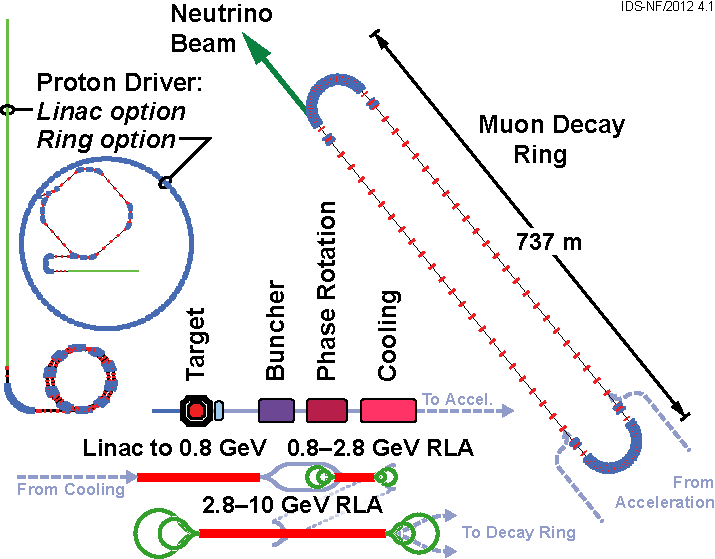
\includegraphics[width=0.9\textwidth]{figures/131112-IDS-NF.pdf}
\caption{Schematic diagram of the Neutrino Factory~\cite{Fix7}.}
\label{fig:nuFact}
\end{figure}

\begin{figure}[h!]
\centering
\includegraphics[width=0.9\textwidth]{figures/rdr-cp-precision-comparison-131216.pdf}
\caption{Expected precision for a measurement of the $\delta_{cp}$ at a Neutrino Factory compared to alternate neutrino oscillation facilities~\cite{Fix7}.}
\label{fig:nuFactExp}
\end{figure}


\textbf{Add in different channels and how it requires a charge identification to be able to identify the various challenge.}

\subsection{NuStorm}

The Neutrino Factory is a complex and expensive facility which requires new technology to be realised. To overcome this a staged approach has been suggested, where each stage would be delivering physics~\cite{Fix7}. The first state in this plan is named nuSTORM (Neutrinos from Stored Muons) with a schematic shown in figure~\ref{fig:nuStorm}. The nuSTORM beam is designed to produce 3.8 GeV/c muons which are injected into a muon storage ring. Compared to the full neutrino factory nuSTORM is expected to have some pions and kaons for the first pass in the storage ring providing some contamination in the final beam producing both neutrinos and anti-neutrinos for both muon and anti-muon modes and thus a near detector is required to measure the flux of both. 

\begin{figure}[h!]
\centering
\includegraphics[width=\textwidth]{figures/nuSTORM_schematic.pdf}
\caption{A schematic of a nuSTORM facility~\cite{Fix7}.}
\label{fig:nuStorm}
\end{figure}

For the both NuFACT and nuSTORM the detector type proposed will be a MIND type, similar to the ones used in CDHSW and MINOS~\cite{NuFACTIDS}.

~\cite{77nustorm}.

\section{Magnetized Iron Neutrino Detectors}\label{subsec:MINDdetector}
\textbf{Correct after Pauls comments and add data.}

Magnetized Iron Neutrino Detectors (MINDs) have been operated in several experiments such as CDHSW~\cite{40CDHSW} and MINOS~\cite{MINOS}. This type of detector, with magnetized steel plates and scintillation plates, is well suited to provide large mass for neutrino experiments and is able to provide momentum measurements by using range and curvature calculations as well as providing charge identification. A MIND type detector has been selected as the baseline detector for a neutrino factory~\cite{ISS, 27Bross}, since it is the cheapest and most effective way of producing a large magnetized volume. This has provided the motivation for creating a prototype detector to perform a number of studies.

Since water Cherenkov and liquid argon detectors have been established or actively studied for future very large scale neutrino oscillation experiments, a MIND type detector is not foreseen to be used as the main interaction medium for any planned upcoming experiments.. A MIND type detector can however be used to provide charge identification of muons if positioned downstream of any neutrino target which is not magnetized.

\if{0}
\textbf{OLD}

\subsubsection{IceCube}
The IceCube observatory~\cite{43IceCube} also exploits the fact that particles produced in neutrino interactions emit Cherenkov photons. The low interaction probability of neutrinos require a large interaction volume. The South Pole offers a large interaction volume with very good optical qualities, using this is possible to instrument cubic kilometres of ice with a rather sparse spacing of detectors. The basic detection unit in IceCube is the digital optical module (DOM). The DOM contains, amount other things a PMT encapsulated in a glass pressure sphere to withstand the extreme pressure in the deep ice. In total 5160 DOMS are deployed, instrumenting a volume of one cubic kilometre of ice and allowing detection of astrophysical neutrinos in the energy range of TeV to PeV.

\begin{figure}
\centering
\includegraphics[width=.5\textwidth]{figures/IceCube.jpeg}
\caption{The IceCube Neutrino Observatory}
\end{figure}
\fi






%==============================================================================


% -----------------------------------------------------------------------------
% Main stuff.

\chapter{WAGASCI + BabyMIND}
\label{c:WAGASCI}

\section{WAGASCI}

A new water-scintillator detector, WAGASCI (WAter- Grid-SCIintilator-Detector) seen in figure~\ref{fig:WAGASCI}, is proposed to reduce the systematic error in the T2K neutrino experiment.
The main goals of the proposed detector are to improve the charge current cross section ratio between water and scintillator targets and to perform high-precision measurement of different charged current neutrino interaction channels.

\begin{figure}[h!]
\centering
\includegraphics[width=\textwidth]{figures/WAGASCI.png}
\caption{The basic structure of the WAGASCI detector including one of the possible designs for the MIND plates.~\cite{30WAGASCI}.}
\label{fig:WAGASCI}
\end{figure}


\subsection{Collaboration}
No idea, is there even an official website?
\subsection{Layout}
Official images?
\subsection{Motivation}
Official paper?

\section{BabyMIND}
\subsection{Collaboration}
Do we have an official list?
\subsection{Layout}
What papers, images can I should I use.
\subsection{Motivation}
In the white paper? LOI.

\chapter{SaRoMaN}
%\chapter{Software development}
\label{c:software}

\section{Introduction}

The software environment used for Baby MIND is the SaRoMaN (Simulation and Reconstruction of Muons and Neutrinos) software suite which is a comprehensive software for MIND/nuSTORM detectors and has been developed at the University of Glasgow over several iterations~\cite{27Bross,  53Laing, 54NUFACT2016Hallsjo}. The software has been expanded to be able to model and simulate a generic detector with limitations in the current implementation of the reconstruction. It includes a complete range of functionality for simulating single particle beams, through GEANT4~\cite{Geant4} or neutrino beams, through GENIE~\cite{Genie}, including geometry design, digitisation and reconstruction through RecPack~\cite{RecPack}. The software suite is also shipped with several analysis code examples written in ROOT~\cite{Root}. It has been created exploiting software engineering and object-oriented technology and implemented in the C++ and Python programming languages. The software is accessible on request from \url{https://lspace.ppe.gla.ac.uk}. 

\section{General structure}
The SaRoMaN software suites main design goal has been to promote modularity, single point of entry and simplicity for the user. With this in mind the SaRoMaN software is split into four main parts which can be replaced or altered independently of the others as long as the input/output flow is conserved. The parts are denoted, wrapper, simulation, digitisation and reconstruction with the flow seen in \FigRef{fig:codeFlow} and a more detailed view in \FigRef{fig:structure}. Each part will be discussed further below.

\begin{figure}[h!]
\centering
\includegraphics[width=\textwidth]{figures/codeFlow.png}
\caption{Code flow of the SaRoMaN software suite all controlled and handled through a wrapper.}
\label{fig:codeFlow}
\end{figure}

\begin{figure}[h!]
\centering
\includegraphics[width=\textwidth]{figures/Software_structure.pdf}
\caption{Code structure of the SaRoMaN software suite all controlled and handled through a wrapper.}
\label{fig:structure}
\end{figure}

%The second simulation etc etc.
%Add diagram of code, structure etc. Perhaps some code and or file structures in the appendix.
%Plot the overlaying idea and structure. Stress modularity, charge, momentum and particle type

\section{Wrapper}
To simplify the installation, compiling and usage of the other parts in the SaRoMaN suite, a wrapper has been developed in the Python programming language. This wrapper, aside from the above, handles all input variables, file names, writing of configuration files, standardisation of magnetic field map and geometry, and data flow between the other parts. 

To simplify for the user, all of the installation, compilation and running are handled through simple command line inputs with the option of more advanced commands being issued through the use of the Python wrapper class. After installation SaRoMaN can be run with some default parameters, a full run diagram can be seen in \FigRef{fig:block}.

\begin{figure}[h!]
\centering
\includegraphics[width=\textwidth]{figures/block.pdf}
\caption{Example of how to run a default simulation.}
\label{fig:block}
\end{figure}

\section{Simulation}
Simulations are used to model how particles will interact with a detector model and what scintillator hits can be expected. The outputs from the simulation include the position of the hit on a bar, the location of a bar, the time of the hit and the amount of energy that was deposited.

The simulation comes with two different modes, neutrino or "single particle". For neutrinos GENIE is first run to generate neutrino events. These events are later populated and the detector constructed through GEANT. In a single particle mode a beam of a single particle type is assumed, GENIE is not called and the simulation and detector construction are handled through GEANT.

A unique feature is that the whole SaRoMaN suite uses a single geometry definition for the whole suite, written in Geometry Description Markup Language (GDML)~\cite{GDML} which is interpreted in GEANT and passed as a simplified .txt file to the reconstruction, which simplifies any changes of the geometry. 

\section{Digitisation}
Digitization is the emulation of the hardware required to build the detector. It needs to handle the response of the electronics and describes the expected output signals, based on input hits in the detector. This is currently done in a simplified way by smearing data with different Poisson distributions as well as handling events which are distinguished by a large time difference. For the Baby MIND detector the algorithms take the horizontal and vertical bar hits and clusters together hits to construct x, y and z positions along with the energy deposition and time to produce physical hit points. The full program flow can be seen in \FigRef{fig:digi}.

As a way to simplify the integration and implementation, the data acquisition (DAQ) used for the different test beams have been implemented in the digitisation as well. In this mode, real data is given as input and only the clustering takes place. Due to the usage of a single geometry, a token simulation has to be run in this mode as well to properly construct the geometry.

To ensure that all further analysis is performed properly, there is no way to distinguish data coming out of the digitisation as being simulated or read in through the DAQ.

One of the most difficult design features of Baby MIND is combining hits from both vertical and horizontal bars. It is possible to get hits which can not be combined without ambiguity. In figure~\FigRef{BarAmbi} it is impossible to distinguished the green hits from each other and the same with the red hits. The current method is for the digitisation to create both hits at all times and these hits being handled by the reconstruction.

\begin{figure}[h!]
\centering
\includegraphics[width=\textwidth]{figures/Digitisation.jpg}
\caption{Program flow for the digitisation.}
\label{fig:digi}
\end{figure}

\begin{figure}[h!]
\centering
\includegraphics[width=0.5\textwidth]{figures/BarsAmbi.jpg}
\caption{}
\label{fig:BarAmbi}
\end{figure}

\subsection{Simulated data}

The digitisation is provided with a .root file containing the following variables, add list? 

Given that the data is assumed to be analysed offline, the first task is to separate any hits into event time windows, where hits can be seen as coming from the same particle. The main difficulty is to allow for the particle to fully traverse the detector and allow delay in electronics response in the time window. This provides a number of hits in several time bins, denoted as events without having use the position information. Add plot, logical flow chart.

After the timing clustering so called 3-d space points are created by combining the vertical and horizontal bar hits for a specific module. These three points are combined to provide an x,y and z coordinate. In this bar coincidence as well as overlap are taken into account as mentioned previously by creating all of the possible points. For this position clustering energy is combined between the individual hits to create a or several clusters with a discrete position, based on bar overlap, deposited energy and time.

The final step in the digitisation is to smear the value of deposited energy and hit time based on measured values of propagation time through the scintillator bars given the simulated hit position and not only the bar position.

\subsection{DAQ}
\textbf{Here or test beam?}

The current DAQ framework for the Baby MIND detector is based on being used offline, processed both after and away from the acquisition.

For simplicity the DAQ converts the acquired data and converts it into the same format as expected from a simulation so that the digitisation can be used in the same way. The main difference is that the smearing used for simulated data is turned off. In this section the DAQ will be discussed. 

Data comes in with files specific for each FEB. This data, has channel number, hit time and hit amplitude. The first step is to convert the data into space-positions, either vertical or horizontal bar position information and z-position, using a database based on FEB, channel number and knowledge of the physical layout of the detector. The second step is ensuring that each hit position, time and amplitude. Step three is to cluster all of the hits in specific time slots, which are equivalent to the event time windows. When this is done several low level filters are performed, to ensure that an event has enough hits to produce atleast four 3-d space positions in a time slot. After these steps the data is equivalent to the data produced by a simulation.

\section{Reconstruction}
The reconstruction takes the digitized hit data and assembles tracks and vertices. The main physics parameters are the momentum as well as the charge of the particle. The main problems occur when there are overlapping hits with multiple occupancy per bar. In this situation, it is difficult to distinguish between valid hits and to extract the momentum of the track and its charge.
The first problem is handled by removing and adding hits and using a $\chi^2$ analysis through a Kalman fitter package, RecPack~\cite{RecPack}, to find the best trajectory that fits all hits.The second problem is solved through various algorithms to estimate the charge and momentum using different fits.

For simplicity the reconstruction currently contains a mode denoted as "test beam" where it does nothing more than writes out the input data into a final .root file.

\subsection{Structure}
The reconstruction software has been structured to ensure that the software is as modular as possible. It is currently based on the Kalman fitter package known as RecPack~\cite{RecPack} to provide both a framework and back bone for handling track objects. It is used for historical reasons, however SaRoMaN would benefit from using a Kalman fitter implementation which is still maintained, development, with few and understood bugs and has documentation.

A Kalman fitter is given an underlying model of the system, in our case knowing that particles travel as helices, and a model of the detector as well as other known inputs to the system to form an estimate of the different states in a way that is better than using only a single measurement. This is particularly well suited in particle physics where random noise is given through multiple scattering. It can also take into account the various energy losses and varying magnetic fields. Through this is can use measurements in different parts of the detector to estimate both how the particle has and will continue its propagation. Compared to other models, a Kalman fitter has no underlying assumption about the errors being Gaussian.

In high energy physics one frequently faces the problem of modeling the evolution of a dynamic system from a set of experimental measurements. Most of reconstruction programs use similar methods. However, in general they are reimplemented for each specific experimental setup. Some examples are fitting algorithms (i.e. Kalman Filter), equations for propagation, random noise estimation (i.e. multiple scattering), model corrections (i.e. energy loss, inhomogeneous magnetic field, etc.), model conversion, etc. Similarly, the data structure (measurements, tracks, vertices, etc.), which can be generalised as well, is not reused in most of the cases. The motivation for using RecPack comes from it combining all of this into a simple software package.

SaRoMaN has been split into first initializing the fitter, then using an initial pattern classification to choose reconstruction mode. Currently particles and showers are identified, but only muon-like particles are reconstructed. In this identification a track is produced along with any off track hits. Finally the fitter performs a final charge and momentum estimate on the track and tries to fit more tracks to the off track hits. If this is a neutrino sample, proton/neutron tracks are only built if it finds an initial muon track.

The test beam mode ignores the event classification and uses the fitter to pass information from input through to the final root file.

The reconstruction has split into several minor tasks.
\begin{itemize}
\item Handling data. Pushing the input data into a final root file.
\item Track building / pattern recognition, given an event, (a time window) can we build a track from this?
\item Fitting, with a candidate track, is it possible to add more hits to the track and make it longer? Find secondary tracks? Also, is it possible to estimate the momentum and charge of the track?
\end{itemize}

%How does the code work? When does the split happen? FitTrack in example Event by event. Goes on into fitter. split test beam or normal mode. Test beam only passes on the data with some minor calculations, straight line fit etc. Build planes. Fill planes with hits. After this, into classifier. In classifier, try to build trajectories. Find single "paths/tracks" if not, handle occupancy. Make a plot of this! Have all of the different modes here. Handle low and normal mode. Use or don't use recpack. Chi square analysis, add hits etc etc.  After classifier do a final fitter and write all of the data into a root file. For neutrinos handle short secondary tracks, atleast check for them. In the current implementation all parts use some part of RecPack. Stress modularity. Plot with flow through reconstruction.

\subsection{Pattern recognition}
The pattern recognition starts by looking at the number of hits for a given event. There are currently two main limitations to if a track can be fitted.
\begin{itemize}
\item At least 4 hits single hits are required to do any form of charge estimation or track building.
\item At least 10 single hits are required to perform a Kalman fitting.
\end{itemize}
Outside of these limitations, currently only muon track fitting has been implemented. The general assumption is that each even will contain at least one muon track followed by other secondary tracks. If this is not the case the event is discarded. The event filtering is done very simply by assuming anything that is not a shower is a muon. Single hits here refers to separable space points meaning that for each z-position there is only one unique hit. The aim of the pattern recognition is to find as many tracks with single hits as possible. In the pattern recognition track are built up from so called track stubs of at least 4 single hits. As soon as a track stub is created other hits can be added onto the track stub to create a final track using $\chi^2$ as a metric. This $\chi^2$ analysis is run through the fitter and requires an initial charge and momentum guess. This means that the best suitable hits are added to the track stub and the other hits saved for use in finding secondary tracks. 

The program flow can be seen as taking in an event worth of hits and returning a number of tracks along with hits which could not be fitted into any track. Each returned track contains only single hits as well as a momentum and charge estimate. The latter two are then improved by the fitter.

%Given an event, a time selection which can be seen as part of a accelerator spill cycle. Is it possible from the ensemble of hits to find a track or several tracks. Currently makes the assumption that tracks will be separable in space for at least 4 points or that there are 4 planes with single track points as to have an initial track to later add more points into.

\subsection{Fitting}
The fitters main job is to build tracks and to estimate the momentum and charge of that track. There are two modes, one main mode for hits with more than 9 hits are passed into the Kalman fitter RecPack. When it is not possible to perform a helical fit and for any track with more than 3 hits, a self implemented lever-arm approach is used. In both cases RecPack is used to build the tracks, however the momentum and charge reconstruction has to be split depending on the possibility of a helical fit or not. The full helix equation seen below, has a total of 9 parameters and takes 10 measurements to be fully fitted.  
\begin{align}
x(t) &= acos(bt+c)+d\\
y(t) &= esin(ft+g) + h\\
z(t) &= kt
\end{align}

The helix can be related to physical quantities as.
%This can also be written in a more helpful way as.
%http://www-jlc.kek.jp/subg/offl/lib/docs/helix_manip/main.html

\begin{align}
x(\phi) &= x_0 + d_p \cos \phi_0 + \frac{\alpha}{\kappa}(\cos \phi_0 - cos(\phi_0 + \phi))\\ 
y(\phi) &= y_0 + d_p \sin \phi_0 + \frac{\alpha}{\kappa}(\sin \phi_0 - cos(\phi_0 + \phi))\\
z(\phi) &= z_0 + d_z - \frac{\alpha}{\kappa} tan \lambda \phi
\end{align}
where $\vec{X} = (x_0, y_0, z_0)$ is the arbitrary helix pivot point, $d_p$ is the distance from the helix to the pivot point in the xy plane, $\phi_0$ is the azimuthal angle from the pivot point with respect tot the helix center, $\kappa$ is the signed reciprocal transverse momentum, $d_z$ is the distance of the helix from the pivot point in the z direction, and $\tan\lambda$ is the dip angle. The deflection angle $\phi$ is measured from the pivot point and specifies the position of the charged particle on the helical track. The variable $\kappa$ can be used to relate to the transverse particle momentum, $P_T$ and relate to the magnetic field as 
\begin{align}
 \kappa &=  Q/P_T \\  
 \rho &=  \alpha/\kappa
 \end{align}
where Q is the particle charge, $\rho$ being the signed radius of the helix, and $\alpha \equiv 1/c B$ being a magnetic-field-dependent constant with c as a constant and B the magnetic field strength. The full particle momentum can be obtained as 
\begin{equation}
\vec{P} = - \frac{Q}{\alpha} \frac{d\vec{X}}{d\phi} = \frac{1}{|\kappa |} 
 \begin{pmatrix}
 -\sin(\phi_0 + \phi)\\
 cos(\phi_0 + \phi)\\
 tan\lambda
 \end{pmatrix}
\end{equation}

In practice, this fit also takes both energy loss in the detector and multiple scattering into account when calculating the $\chi^2$ values when fitting the parameters. 

This motivates the requirement for two different modes. If a helical fit is possible RecPack performs the fitting and returns a final fitted helix, within provided measurement errors, with a momentum and charge estimate.

If a helical fit is not possible, denoted the low momentum case, several different algorithms are used.

The fitting is performed in a usual Kalman way by using this underlying equation and assuming each measurement point has some error.
Each measurement point $\vec{X}$ is related to the next through extrapolating the helical equation and assuming an error: $\vec{X_{k+1}} = \vec{F_{k+1,k}}\vec{X_k} + \vec{w_k}$. 
the output is then given as: $\vec{Y_{k}} = \vec{H_{k}}\vec{X_k} + \vec{v_k}$
The helical equation goes into forming the matrix F and H.

\subsection{Low momentum algorithms}
The force applied to a particle travelling through a magnetic field is given by the Lorentz force:
\begin{equation}
\vec{F}=q\frac{\vec{v}\times\vec{B}}{c}
\end{equation}
where c is the speed of light in vacuum, v is the velocity, q the charge and B the magnetic field vector.

Using Newtons second law one produces the following differential vector equation.
\begin{equation}
\vec{F}=m\vec{a}=m\dot{\vec{v}}=q\frac{\vec{v}\times\vec{B}}{c}
\end{equation}
The solution to this equation is given by:
\begin{equation}
\vec{P}=m\vec{a}=m\vec{v}=q\frac{\vec{l}\times\vec{B}}{c}
\end{equation} 
where P is the momentum of the particle and $\vec{l}=\vec{X}-\vec{X_0}$ is a vector containing the lengths traversed through the magnetic field.

Using the definition of the cross-product, writing this as a scalar equation, using the small angle approximation and writing using S.I. units produces the normally recognisable equation
\begin{equation}
P = 0.3 QB_\bot \frac{|\vec{l}|}{\theta}=0.3 QB_\bot R
\end{equation}
where P is the momentum in MeV/c, the charge Q in in units of e, the magnetic field strength B is in T and the radius of curvature R is in cm. This is only one way of deriving the relation, but it is one of the main equations used for momentum reconstruction in SaRoMaN. The charge is then reconstructed using $P/|P|$ \textbf{Figure of one bending in first plane in mind.}

\begin{figure}[h!]
\centering
\includegraphics[width=0.5\textwidth]{figures/lowP/scattering.jpeg}
\caption{}
\label{fig:Scattering}
\end{figure}

A previous study performed in the collaboration showed that the best best way of evaluating the charge comes from comparing both the first and second bending in the detector using two different distributions to handle the scattering.

\begin{figure}[h!]
\centering
\includegraphics[width=0.5\textwidth]{figures/lowP/null.jpg}
\caption{}
\label{fig:NullHyp}
\end{figure}

Using the distribution of multiple scattering angles and the notation in \FigRef{fig:NullHyp}, the choice is taken as. 

Reconstruct $\mu^-$ if 
\begin{equation}
\frac{f_{\mu^-}(\Delta_1)}{f_{\mu^+}(\Delta_1)} > \frac{f_{\mu^+}(\Delta_2)}{f_{\mu^-}(\Delta_2)}
\end{equation}
and as $mu^+$ if
Reconstruct $\mu^-$ if 
\begin{equation}
\frac{f_{\mu^+}(\Delta_1)}{f_{\mu^-}(\Delta_1)} > \frac{f_{\mu^-}(\Delta_2)}{f_{\mu^+}(\Delta_2)}
\end{equation}

The bending angles are calculated from both measurement planes, (or only one if not possible) and tested against a null-hypothesis of having deflection from only multiple scattering 

%link from http://pdg.lbl.gov/2000/passagerpp.pdf
%Also, look at mind_rec/detector.c

multiple scattering  through small angles, the angle is given by, taken from pdg link
\begin{equation}
\theta_0 = \frac{13.6 MeV}{\beta cp} z \sqrt{x/X_0}[1+0.038\ln(x/X_0)]
\end{equation}
where p is the momentum, $\beta c$ the velocity, z the charge number of the incident particle and $x/X_0$ is the thickness of the scattering medium in radiation lengths.

The probability is calculated as 1/2pi exp -(scattering angle +- total bending angle) etc. check code.





Use the angles to and probability to calculate the charge. Momentum currently from range. Seems better.

Probability of angle from multiple scattering, or from magnetic field. 

Momentum comes from the range calculation, see detector layout. Major gaps in monument,  Potentially could and perhaps should use range momentum as long as tracks stop in detector. Problem with steps, helix better.



This seems to be the best approach. If this for some reason fails it goes on to a final attempt.

Quadratic fit, given few hits, try to fit to return charge. Use this only for charge. Momentum from range momentum.

\subsection{Performance}
During development of SaRoMaN two main metrics were used to evaluate performance, charge reconstruction efficiency and track reconstructed efficiency. These metrics provide information about how many simulated tracks can be reconstructed and how many of those reconstructed tracks have the correct charge. This is done for muons of both charges and different momentum values.

Performance will be shown for the initial and proposed layout, for which the software algorithms were designed, the layout required for the text beam due to construction constraints and a final study based on the layout used for the WAGASCI detector layout. The main difference between the initial and test beam layout is removing the initial measurement point D0, restructuring  the layout and adding gaps between each of the blocks. This was done from a constructional not a physics motivation.

The charge identification is however improved when utilizing a measurement point from a neutrino target such as the WAGASCI, however this will reduce the lower limit of reconstruction since the muons must traverse the material of the WAGASCI. 

\textbf{Perhaps momentum rec plots as well? Look at old material/collaboration meeting 2 with pull and residuals.}
\textbf{One plot comparing all of these? Can we compare them? Lower momentum due to TASD?}

\begin{figure}[h!]
\centering
\includegraphics[width=0.48\textwidth]{figures/oldStudies/oldMIND.png}
\includegraphics[width=0.48\textwidth]{figures/oldStudies/MINDetam.jpeg}
\caption{(Left) Image of the initial Baby MIND layout. (Right) The current Baby MIND layout. The main differences consists of removing the first scintillator plane, some different layout in the middle blocks and removed the final scintillator plane.}
\label{fig:oldMIND}
\end{figure}

\begin{figure}[h!]
\centering
\includegraphics[width=0.48\textwidth]{figures/oldStudies/oldChargeID.png}
\includegraphics[width=0.48\textwidth]{figures/oldStudies/oldRecEff.png}
\caption{Metric plots of the initial Baby MIND layout with all algorithms adjusted to utilize this layout.}
\label{fig:oldMIND2}
\end{figure}

\begin{figure}[h!]
\centering
\includegraphics[width=0.48\textwidth]{figures/oldStudies/FullChargeID.pdf}
\includegraphics[width=0.48\textwidth]{figures/oldStudies/FullFitted.pdf}
\caption{Metric plots of the current Baby MIND layout.}
\label{fig:TestBeamMIND2}
\end{figure}

Give for different layouts. The initial, well worked. Then work down to the test beam layout and perhaps the latest J-parc layout? 

Charge id, fitting id, momentum pulls and so on.
Look at muons/pions. pure beams with and without TASD/WAGASCI. Especially test beam layout and J-Parc.

Add in the new layout studies?

Quite good, add that charge ID is about x for range y and so on.  Could be improved by changing layout, perhaps even tweaking algorithms etc etc but want to keep generic algorithms to handle different designs.

\textbf{Perhaps cite my Uppsala proceedings?} When it is citable.

\subsection{DAQ}
Add data plots perhaps? Not sure what goes here.

Should I add details about the data format?

Explain how the unpacking works, the main data structure assumed in the electronics. The main problem with the data structure, how it is not aimed to work online. 

Read and use documentation from Yordan Ivanov Karadzhov. Also look at what Aleksander, Sascha has done and what is in the code.


\subsection{Particle identification}
Machine learning through the Toolkit for Multivariate Data Analysis with ROOT (TMVA)~\cite{TMVA}. Add some small part about what ML is and TMVA as well as some minor plots showing performances.

So far have results for $\mu^+/\mu^-$ in a background of  $\pi^+/\pi^-$.

Currently found that the best method, however many perform similarly, is MLPBNN, Multilayer perceptron (neutral network) with BFGS training method, similar to gradient decent or quasi-Newton method, and bayesian regulator.

\subsection{Analysis software}
Start by combining, if needed, several root files. Continue by choosing interesting root branches, with or without filtering/cutting the data.
add analysis flows. What is a normal data flow? Add parts to appendix, more data etc etc etc.

Final root file, read in trees, filter out bad events, if any. Compare apples to apples. 



\input{"5-Testbeam/testbeam.tex"}

\chapter{Neutrino interaction studies}
\label{c:neutrino}

Lab report again, trying to estimate cross-section of interactions. Why? Need it to improve oscillation measurements. Using simulations of muon neutrinos from simulation. What is done, what cuts? How Do we calculate cross-sections? Angular acceptance, look at what Marc has done, do similar things and further the calculations.

Discuss what to expect, what kind of interactions could happen in the TASD/WAGASCI? What could be seen? What information? Baby MIND can also have interactions, which ones would be visible? Can reconstruct muons in Baby MIND, electrons and pions visible and potentially reconstructable, but not now.

\section{Muon charge current quasi-elastic}

Acceptance study, detector layout. Beam settings? Add charge reconstruction, momentum reconstruction. Particle ID? also need interaction ID from TMVA.

Different size gap, different detector layout both early/testbeam and new at Japan.


Cross-section studies. Look at what Marc has done! 

Discuss with paul what and how to do cross-section measurements.

\subsection{Neutrino interactions in TASD + Baby MIND}

\subsubsection{Interactions in TASD}

\subsubsection{Interactions in Baby MIND}

\subsection{Neutrino interactions in WAGASCI + Baby MIND}

\subsubsection{Interactions in Baby MIND}

\subsubsection{Interactions in the ful WAGASCI}

\subsubsection{Simulations vs data}


%\subsection{GAr + BabyMIND}
%\subsubsection{Analysis Simulations}
%\subsection{TASD + BabyMIND}
%\subsubsection{Analysis Simulations}
%\subsection{Full WAGASCI}
%\subsubsection{Analysis with Simulations}
%\subsubsection{Simulations vs data}

\section{Electron charge current quasi-elastic}



\input{"7-NSI/NSI.tex"}

\chapter{Conclusions and Outlook}
\label{c:conclusion}

\section{Baby MIND}

\section{WAGASCI}

\section{Software}

%\section{Project management}

\section{Machine learning in physics}

\section{Neutrino physics}






%\input{"2-main/babyMINDintro.tex"}

%\input{"2-main/babyMINDdata.tex"}

%\input{"2-main/Phenom.tex"}


% -----------------------------------------------------------------------------
\appendix

% For the year 2 review, need "current results" and outline for next 12 months.


%\chapter{Current results Year2}
\label{a:appendix}

From last year the software has been completed and can handle neutrino and muon beam events in a generic MIND type detector. The main problem used to be how to handle multiple hit occupancy but this changed to be an issue with momentum reconstruction. The problem arose from bugs and incorrect use of the third-party software RecPack which is a kalman filter fitter. There are still some issues with the pull plots however it has been improved considerately and the bugs are understood. The main issue seems to be an underestimation of the error for low momentum values. See figures~\ref{fig:mommu}, ~\ref{fig:momantimu}, ~\ref{fig:meanmu}, ~\ref{fig:meanantimu}, ~\ref{fig:sigmamu}, ~\ref{fig:sigmaantimu}.

Figure~\ref{fig:fullrec} shows the current reconstruction efficiency, using simulated data in Baby MIND, defined as the number of reconstructed tracks from the number of identified trajectories and reconstructed with a momentum non-zero to remove errors in the code. For a single muon beam, the efficiency is more than 95\% for the expected full range (0.2-10 GeV/c). Figure~\ref{fig:fullcharge} shows the current charge identification efficiency, which is defined as the number of tracks with the correctly assigned charge out of all the reconstructed trajectories.  For a single muon beam, the efficiency is more than 95\% above 0.8 GeV/c and above 80\% in the region 0.2-0.8GeV/c.

\begin{figure}[h!]
	\begin{minipage}{0.49\linewidth}
		\centerline{\includegraphics[width=0.9\linewidth]{figures/FullFitted.pdf}}
		%\caption[]{ Reconstruction efficiency: out of identified trajectories, how many are reconstructed?}
			\caption[]{Reconstruction efficiency for a single muon beam}
		\label{fig:fullcharge}
	\end{minipage}
	\hfill
	\begin{minipage}{0.49\linewidth}
		\centerline{\includegraphics[width=0.9\textwidth]{figures/FullChargeID.pdf}}
		\caption[]{Charge identification efficiency for a single muon beam}
		%	\caption[]{Charge identification efficiency: out of reconstructed trajectories, how many are identified with the correct charge?
		\label{fig:fullrec}
	\end{minipage}
\end{figure}


\begin{figure}[h!]
	\begin{minipage}{0.49\linewidth}
		\centerline{\includegraphics[width=0.9\linewidth]{figures/mupull.pdf}}
		%\caption[]{ Reconstruction efficiency: out of identified trajectories, how many are reconstructed?}
			\caption[]{Momentum pull plot for a single $\mu^-$ beam}
		\label{fig:mommu}
	\end{minipage}
	\hfill
	\begin{minipage}{0.49\linewidth}
		\centerline{\includegraphics[width=0.9\textwidth]{figures/antimupull.pdf}}
		\caption[]{Momentum pull plot for a single $\mu^+$ beam}
		%	\caption[]{Charge identification efficiency: out of reconstructed trajectories, how many are identified with the correct charge?
		\label{fig:momantimu}
	\end{minipage}
\end{figure}

\begin{figure}[h!]
	\begin{minipage}{0.49\linewidth}
		\centerline{\includegraphics[width=0.9\linewidth]{figures/mumean.pdf}}
		%\caption[]{ Reconstruction efficiency: out of identified trajectories, how many are reconstructed?}
			\caption[]{The mean evolution of the pull plot for a single $\mu^-$ beam}
		\label{fig:meanmu}
	\end{minipage}
	\hfill
	\begin{minipage}{0.49\linewidth}
		\centerline{\includegraphics[width=0.9\textwidth]{figures/antimumean.pdf}}
		\caption[]{The mean evolution of the pull plot for a single $\mu^+$ beam}
		%	\caption[]{Charge identification efficiency: out of reconstructed trajectories, how many are identified with the correct charge?
		\label{fig:meanantimu}
	\end{minipage}
\end{figure}

\begin{figure}[h!]
	\begin{minipage}{0.49\linewidth}
		\centerline{\includegraphics[width=0.9\linewidth]{figures/musigma.pdf}}
		%\caption[]{ Reconstruction efficiency: out of identified trajectories, how many are reconstructed?}
			\caption[]{The sigma evolution of the pull plot for a single $\mu^-$ beam}
		\label{fig:sigmamu}
	\end{minipage}
	\hfill
	\begin{minipage}{0.49\linewidth}
		\centerline{\includegraphics[width=0.9\textwidth]{figures/antimusigma.pdf}}
		\caption[]{The sigma evolution of the pull plot for a single $\mu^+$ beam}
		%	\caption[]{Charge identification efficiency: out of reconstructed trajectories, how many are identified with the correct charge?
		\label{fig:sigmaantimu}
	\end{minipage}
\end{figure}

During June-July 2016 a test beam was performed to characterise the readout system, data acquisition (DAQ) and electronics to be used in the Baby MIND detector. The test beam was at the T9 beam of the East Area, operating at the Proton Synchrotron (PS) at CERN. A Totally Active Scintillation Detector (TASD)~\ref{fig:AIDA} constructed under the AIDA project (Advanced European Infrastructures for Detectors at Accelerators) was used to test the readout system, electronics, DAQ and reconstruction software. For the beam test, twelve planes, consisting of 16 scintillator bars $10\times 10\times 1000$~mm$^3$, read out on both sides by S12571-025C Hamamatsu MPPCs  along alternating $x$ and $y$ directions were instrumented (a total of 384 MPPCs). The beam consisted of muons and pions from $\sim$200~MeV/c up to 10~GeV/c. Figure~\ref{fig:AIDA} shows a schematic of the TASD and figure~\ref{fig:beamProfile} shows the evolution of the beam profile as measured by the TASD during the test beam and reconstructed with the SaRoMan software. 

\begin{figure}[h]
	\begin{minipage}{0.39\linewidth}
		\centerline{\includegraphics[width=0.9\linewidth]{Figures/AIDA.png}}
		\caption[]{The TASD with the instrumented bars visualised.}
		\label{fig:AIDA}
	\end{minipage}
	\hfill
	\begin{minipage}{0.59\linewidth}
		\centerline{\includegraphics[width=\textwidth, trim = 5cm 5cm 5cm 5cm]{Figures/beamPlot.pdf}}
		\caption[]{Beam profile measured by the TASD.}
		\label{fig:beamProfile}
	\end{minipage}
\end{figure}

Unfortunately for neutrino tracks it would be beneficial to perform simulations with the WAGASCI + Baby MIND but the WAGASCI design has not yet been shared from that collaboration. Instead these neutrino track simulations have been performed using the TASD as a target and then Baby MIND as a muon spectrometer behind it, see~\ref{fig:event} figure~\ref{fig:schematic}. Also for visualization a sample event has been added. The efficiency plots provided,figures~\ref{fig:numufitted} ,~\ref{fig:numucharge},~\ref{fig:antinumufitted} and ~\ref{fig:antinumucharge}, require more data to be fully understood, they do however look promising. Something which needs to be further understood is the pull plots which may indicate an issue for the momentum reconstruction, figures~\ref{fig:numumom}  and ~\ref{fig:antinumumom}, to handle tracks which start off at an angle compared to the beam direction.

\begin{figure}[h!]
	\begin{minipage}{0.49\linewidth}
		\centerline{\includegraphics[width=0.9\linewidth]{figures/mindSide.jpeg}}
		%\caption[]{ Reconstruction efficiency: out of identified trajectories, how many are reconstructed?}
			\caption[]{A schematic for the TASD + babyMIND detector}
		\label{fig:schematic}
	\end{minipage}
	\hfill
	\begin{minipage}{0.49\linewidth}
		\centerline{\includegraphics[width=0.9\textwidth]{figures/muCCQEorigin.pdf}}
		\caption[]{Example of a $\mu^{-}$ CCQE event which interacts in the TASD shown in in Y-Z profile. }
		%	\caption[]{Charge identification efficiency: out of reconstructed trajectories, how many are identified with the correct charge?
		\label{fig:event}
	\end{minipage}
\end{figure}


\begin{figure}[h!]
	\begin{minipage}{0.49\linewidth}
		\centerline{\includegraphics[width=0.9\linewidth]{figures/muNeutrinoFitted.pdf}}
		%\caption[]{ Reconstruction efficiency: out of identified trajectories, how many are reconstructed?}
			\caption[]{Reconstruction efficiency for a single $\nu_{\mu}$ beam}
		\label{fig:numufitted}
	\end{minipage}
	\hfill
	\begin{minipage}{0.49\linewidth}
		\centerline{\includegraphics[width=0.9\textwidth]{figures/muNeutrinochargeID.pdf}}
		\caption[]{Charge identification efficiency for a single  $\nu_{\mu}$ beam}
		%	\caption[]{Charge identification efficiency: out of reconstructed trajectories, how many are identified with the correct charge?
		\label{fig:numucharge}
	\end{minipage}
\end{figure}

\begin{figure}[h!]
	\begin{minipage}{0.49\linewidth}
		\centerline{\includegraphics[width=0.9\linewidth]{figures/antimuNeutrinoFitted.pdf}}
		%\caption[]{ Reconstruction efficiency: out of identified trajectories, how many are reconstructed?}
			\caption[]{Reconstruction efficiency for a single $\bar{\nu_{\mu}}$ beam}
		\label{fig:antinumufitted}
	\end{minipage}
	\hfill
	\begin{minipage}{0.49\linewidth}
		\centerline{\includegraphics[width=0.9\textwidth]{figures/antimuNeutrinochargeID.pdf}}
		\caption[]{Charge identification efficiency for a single $\bar{\nu_{\mu}}$ beam}
		%	\caption[]{Charge identification efficiency: out of reconstructed trajectories, how many are identified with the correct charge?
		\label{fig:antinumucharge}
	\end{minipage}
\end{figure}

\begin{figure}[h!]
	\begin{minipage}{0.49\linewidth}
		\centerline{\includegraphics[width=0.9\linewidth]{figures/muNeutrinoPull.pdf}}
		%\caption[]{ Reconstruction efficiency: out of identified trajectories, how many are reconstructed?}
			\caption[]{Momentum pull plot for a single $\nu_{\mu}$ beam}
		\label{fig:numumom}
	\end{minipage}
	\hfill
	\begin{minipage}{0.49\linewidth}
		\centerline{\includegraphics[width=0.9\textwidth]{figures/antimuNeutrinoPull.pdf}}
		\caption[]{Momentum pull plot for a single $\bar{\nu_{\mu}}$ beam}
		%	\caption[]{Charge identification efficiency: out of reconstructed trajectories, how many are identified with the correct charge?
		\label{fig:antinumumom}
	\end{minipage}
\end{figure}


\chapter{Presented last year}

\section{Presented as Future work last year}
\subsection{Software}
The largest task is to improve the reconstruction algorithms to better classify the events and identify both the momentum and charge. 
Current results seem to show that the main issue is to choose the optimum hits when there is multiple occupancy.

This was improved and corrected in time for the testbeam performed in June of last year.

\subsection{Hardware}
The electronics has been developed at the University of Geneva and will be tested at two test beams in June and July 2016. The current plan is to travel to CERN in June to perform tests with the electronics, to characterise the electronics in the laboratory and in the test beam and to emulate it in the digitization software.

This was tested and the digitization software confirmed with the acquisition of testbeam data.

\subsection{Physics performance}
The main goal is to establish the performance of a MIND type detector in terms of position, angle, momentum and energy resolution and to characterise the particle identification and charge separation. 
Another goal is to benchmark MIND simulations and reconstruction algorithms and compare them with experimental results.

From previous MIND type detectors studies carried out in the context of the Neutrino Factory~\cite{25NUfact}, charge current interactions are of the most interest for a MIND detector since they leave a clearer muon track. Reconstructions of electron tracks become more complex due to much shorter tracks and their similarity to hadronic showers. More detailed tests of electron beams will lead to further understanding of such events.

This is still ongoing. Neutrino tracks can be reconstructed in SaRoMaN, however many bugs have been discovered and have taken more time than expected.

\subsection{Neutrino interaction physics}
The ultimate goal of the research is to characterise neutrino interactions in the WAGASCI detector, identified using Baby MIND to determine the expected cross-section ratio between CC events in water and in carbon. 

This was not achieved and is still seen as a goal to be achieved in August when the detector will be shipped to Japan.

\section{Outline for the "last" 12 months}
\subsection{Software objectives}
\begin{itemize}
\item Launch a complete version of the SaRoMaN software package by June 2016.
\item Integrate the SaRoMaN and WAGASCI software packages by September 2016.
\end{itemize}
\subsection{Physics objectives}
\begin{itemize}
\item Perform physics studies of non-standard neutrino interactions (NSI) by October 2016.
\item Analysis of test beam at CERN by October 2016.
\item Perform neutrino cross-section studies with WAGASCI by February 2017.
\item Perform full Baby MIND beam tests characterization by June 2017.
\end{itemize}
\subsection{Hardware objectives}
\begin{itemize}
\item Perform electronics Front End Board beam test at CERN by July 2016.
\item Finalize Baby MIND by February 2017.
\end{itemize}

Most of these goals were achieved. SaRoMaN has been launched as a complete version and was launched on time. Unfortunately the WAGASCI collaboration has not shared their software so no integration has been made. NSI studies have not been conducted since unfortunately the collaboration with Durham has not been worked at. The electronics test beam and test beam analysis were performed on time. The full Baby MIND will be characterised this June and the design was finalised now in April 2017. Unfortunately neutrino cross-section studies with WAGASCI has not been started since the design has not been fully shared. However they were stated in January with another target design. Several bugs were discovered during these studies, this combined with time spend on other hardware related studies meant that the studies have not yet been completed but they will be completed by September 2017.

\chapter{Outline for the next 12 months}
\section{Objectives}
\label{a:objectives}
\subsection{Software objectives}
\begin{itemize}
\item Improve the SaRoMaN package reconstruction for Neutrino events by September 2017.
\end{itemize}
\subsection{Physics objectives}
\begin{itemize}
\item Perform physics studies of non-standard neutrino interactions (NSI) by October 2017.
\item Analysis of second test beam at CERN by October 2017.
\item Perform neutrino cross-section studies with WAGASCI by December 2017.
\item Perform neutrino cross-section studies with data from WAGASCI by March 2018.
\end{itemize}

\section{Future work}
\subsection{Physics performance}
The main goal is to establish the performance of a MIND type detector in terms of position, angle, momentum and energy resolution and to characterise the particle identification and charge separation. 
Another goal is to benchmark MIND simulations and reconstruction algorithms and compare them with experimental results.

From previous MIND type detectors studies carried out in the context of the Neutrino Factory~\cite{25NUfact}, charge current interactions are of the most interest for a MIND detector since they leave a clearer muon track.

This is still ongoing. Neutrino tracks can be reconstructed in SaRoMaN, however many bugs have been discovered and have taken more time than expected.

\subsection{Neutrino interaction physics}
The ultimate goal of the research is to characterise neutrino interactions in the WAGASCI detector, identified using Baby MIND to determine the expected cross-section ratio between CC events in water and in carbon. 


\section{Gantt chart}

Figure~\ref{fig:Gantt} shows a combined chart of the timeline for Baby MIND and for what conferences I will be aiming for and where I will be. Combined with the objectives given in section~\ref{a:objectives} provides a good plan and outline for the next 6 months.

\begin{figure}[h!]
\centering
\includegraphics[width=\textwidth]{figures/Gantt.png}
\caption{A Gantt chart for the next 12 months.}
\label{fig:Gantt}
\end{figure}



%INCLUDE NEW Gantt chart.
%\begin{figure}[h!]
%\centering
%\includegraphics[width=\textwidth]{ghant.pdf}
%\caption{A Gantt chart for the next 12 months.}
%\label{fig:Gantt}
%\end{figure}



% -----------------------------------------------------------------------------
\newpage

%\fi

\input{"footer.tex"}

